%\subsection{Design in-the-large}
%C-IDM schema

%\subsection{Abstract pages}

%\subsection{Wireframes}

%\subsection{Database}
%DB Design schema(?)

\section{Design-in-the-large}
\subsection{C-IDM}
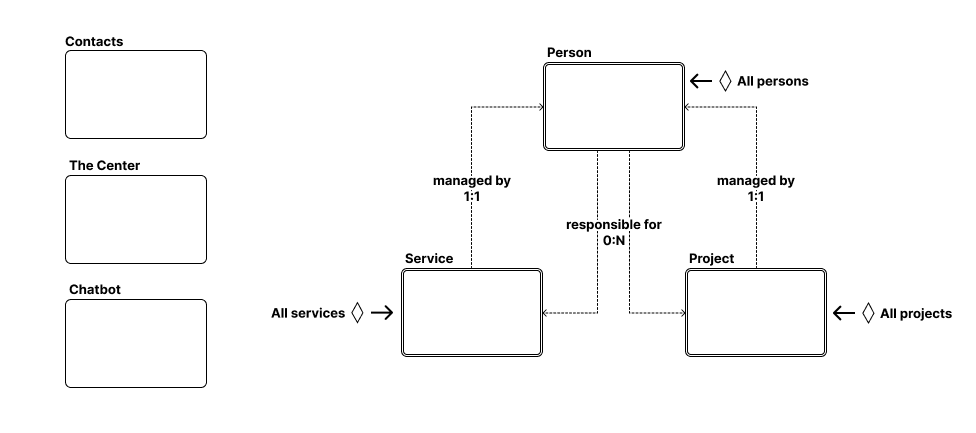
\includegraphics[width=1\linewidth]{img/design-document/C-IDM.png}

\section{Content-in-the-small}
\subsection{Content Tables}

%Kind Of Topic: Person
\begin{tabular}{ |p{5cm}|p{6cm}| }
    \hline
    \multicolumn{2}{|l|}{\textbf{KIND OF TOPIC: Person}} \\
    \hline
    Person Name & text \\
    \hline
    Person Education & text \\
    \hline
    Person Main Expertise & text \\
    \hline
    Person Main Role & text \\
    \hline
    List of Managed Activities & [Service Name, Project Name]\\
    \hline
\end{tabular}

%Kind Of Topic: Service
\begin{tabular}{ |p{5cm}|p{6cm}| }
    \hline
    \multicolumn{2}{|l|}{\textbf{KIND OF TOPIC: Service}} \\
    \hline
    Service Name & text \\
    \hline
    Service Responsible & Person Name \\
    \hline
    Service Date & Date \\
    \hline
    Service Description & text \\
    \hline
    List of Testimonials & [User Name, User Image, User Text] \\
    \hline
\end{tabular}

%Kind Of Topic: Project
\begin{tabular}{ |p{5cm}|p{6cm}| }
    \hline
    \multicolumn{2}{|l|}{\textbf{KIND OF TOPIC: Project}} \\
    \hline
    Project Name & text \\
    \hline
    Project Responsible & Person Name \\
    \hline
    Project Starting Date & date \\
    \hline
    Project Logo & image \\
    \hline
    Project Description & text\\
    \hline
\end{tabular}

%Topic: Chat Bot
\begin{tabular}{ |p{5cm}|p{6cm}| }
    \hline
    \multicolumn{2}{|l|}{\textbf{TOPIC: Chat Bot}} \\
    \hline
    User Input & text \\
    \hline
    Bot Answer & text \\
    \hline
\end{tabular}

%Topic: Contacts
\begin{tabular}{ |p{5cm}|p{6cm}| }
    \hline
    \multicolumn{2}{|l|}{\textbf{TOPIC: Contacts}} \\
    \hline
    UsefulContacts & [Telephone Number, Name]\\
    \hline
\end{tabular}

%Group of Topics: All Services
\begin{tabular}{ |p{5cm}|p{6cm}| }
    \hline
    \multicolumn{2}{|l|}{\textbf{GROUP OF TOPICS: All Services}} \\
    \hline
    Group Title & "Our Services" \\
    \hline
    Services & [Service Title, Service Image, Service Description] \\
    \hline
\end{tabular}

%Group of Topics: All Projects
\begin{tabular}{ |p{5cm}|p{6cm}| }
    \hline
    \multicolumn{2}{|l|}{\textbf{GROUP OF TOPICS: All Projects}} \\
    \hline
    Group Title & "Our Projects" \\
    \hline
    Services & [Project Name, Project Image, Project Description] \\
    \hline
\end{tabular}

\pagebreak
\section{Final Commented Screenshots}

%Homepage
\subsection{Homepage}
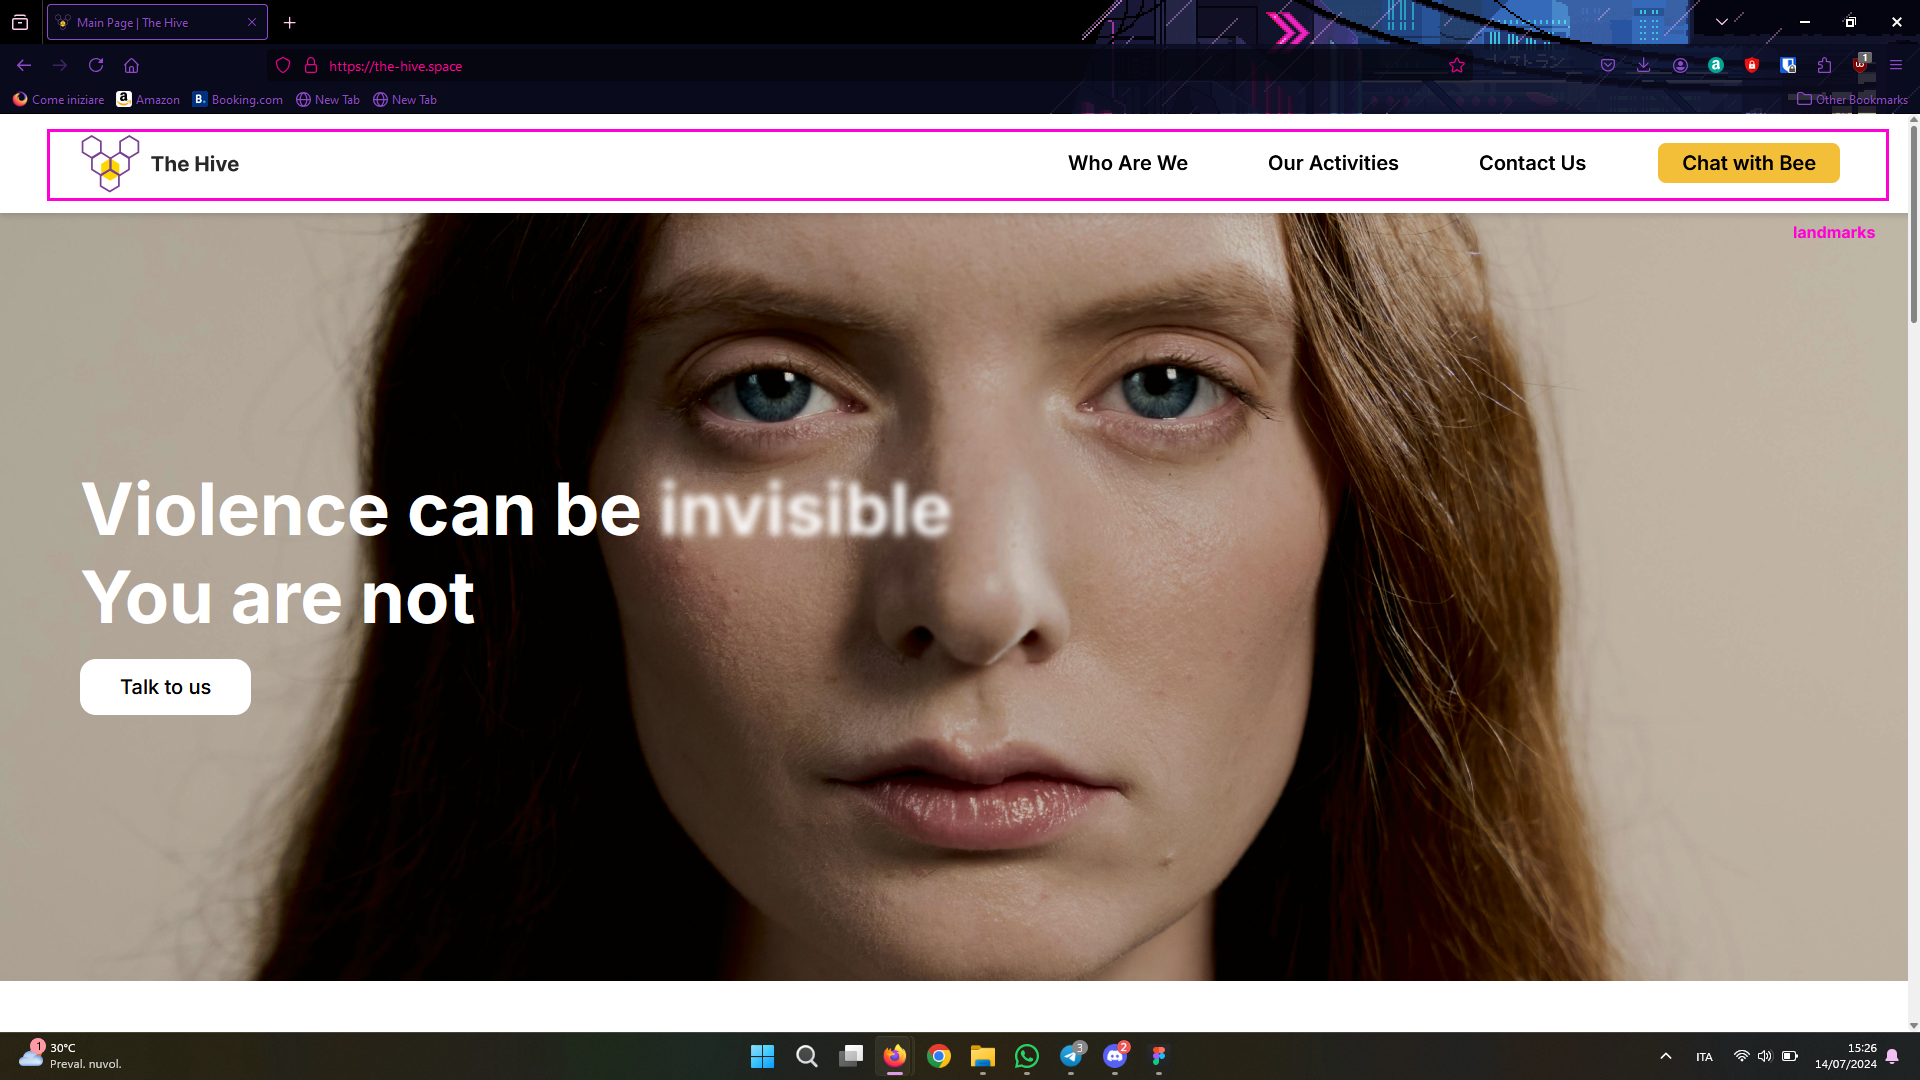
\includegraphics[width=0.5\linewidth]{img/design-document/website-screenshots/homepage-1.png}
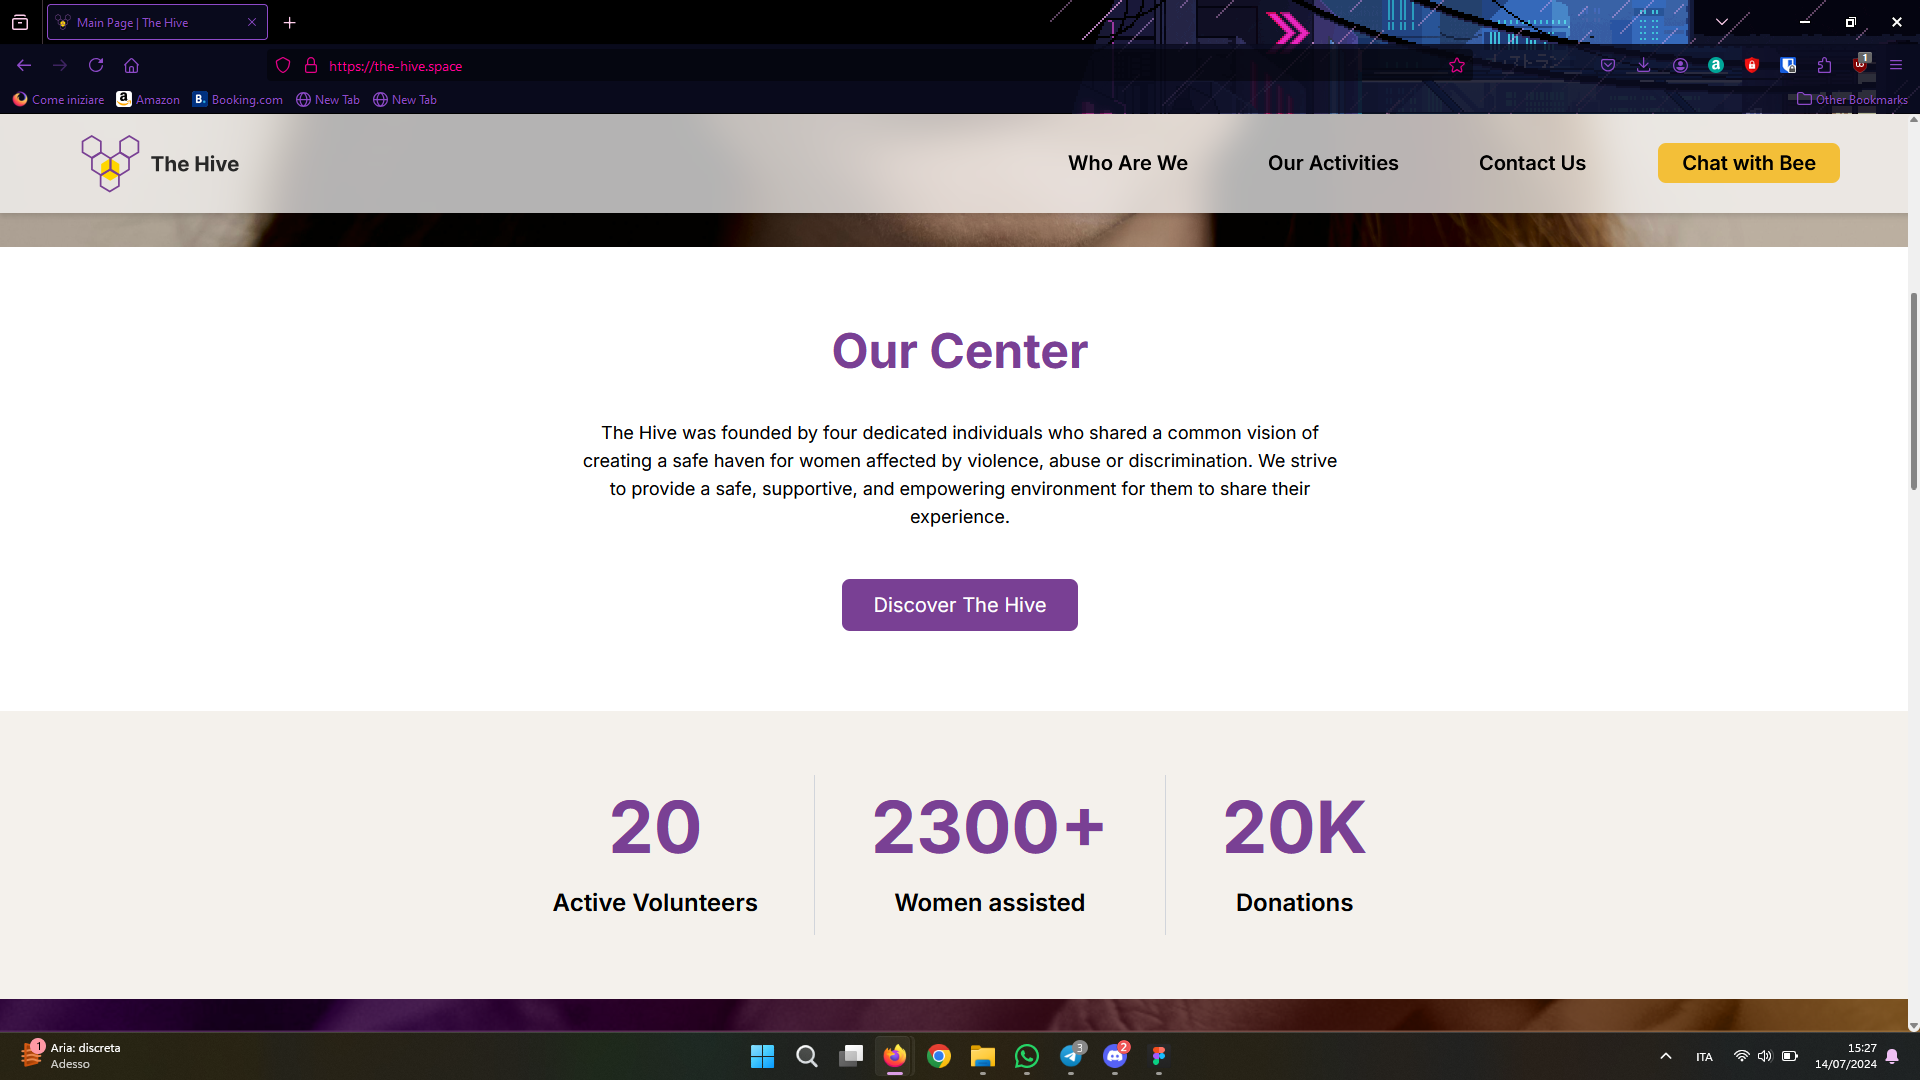
\includegraphics[width=0.5\linewidth]{img/design-document/website-screenshots/homepage-2.png}
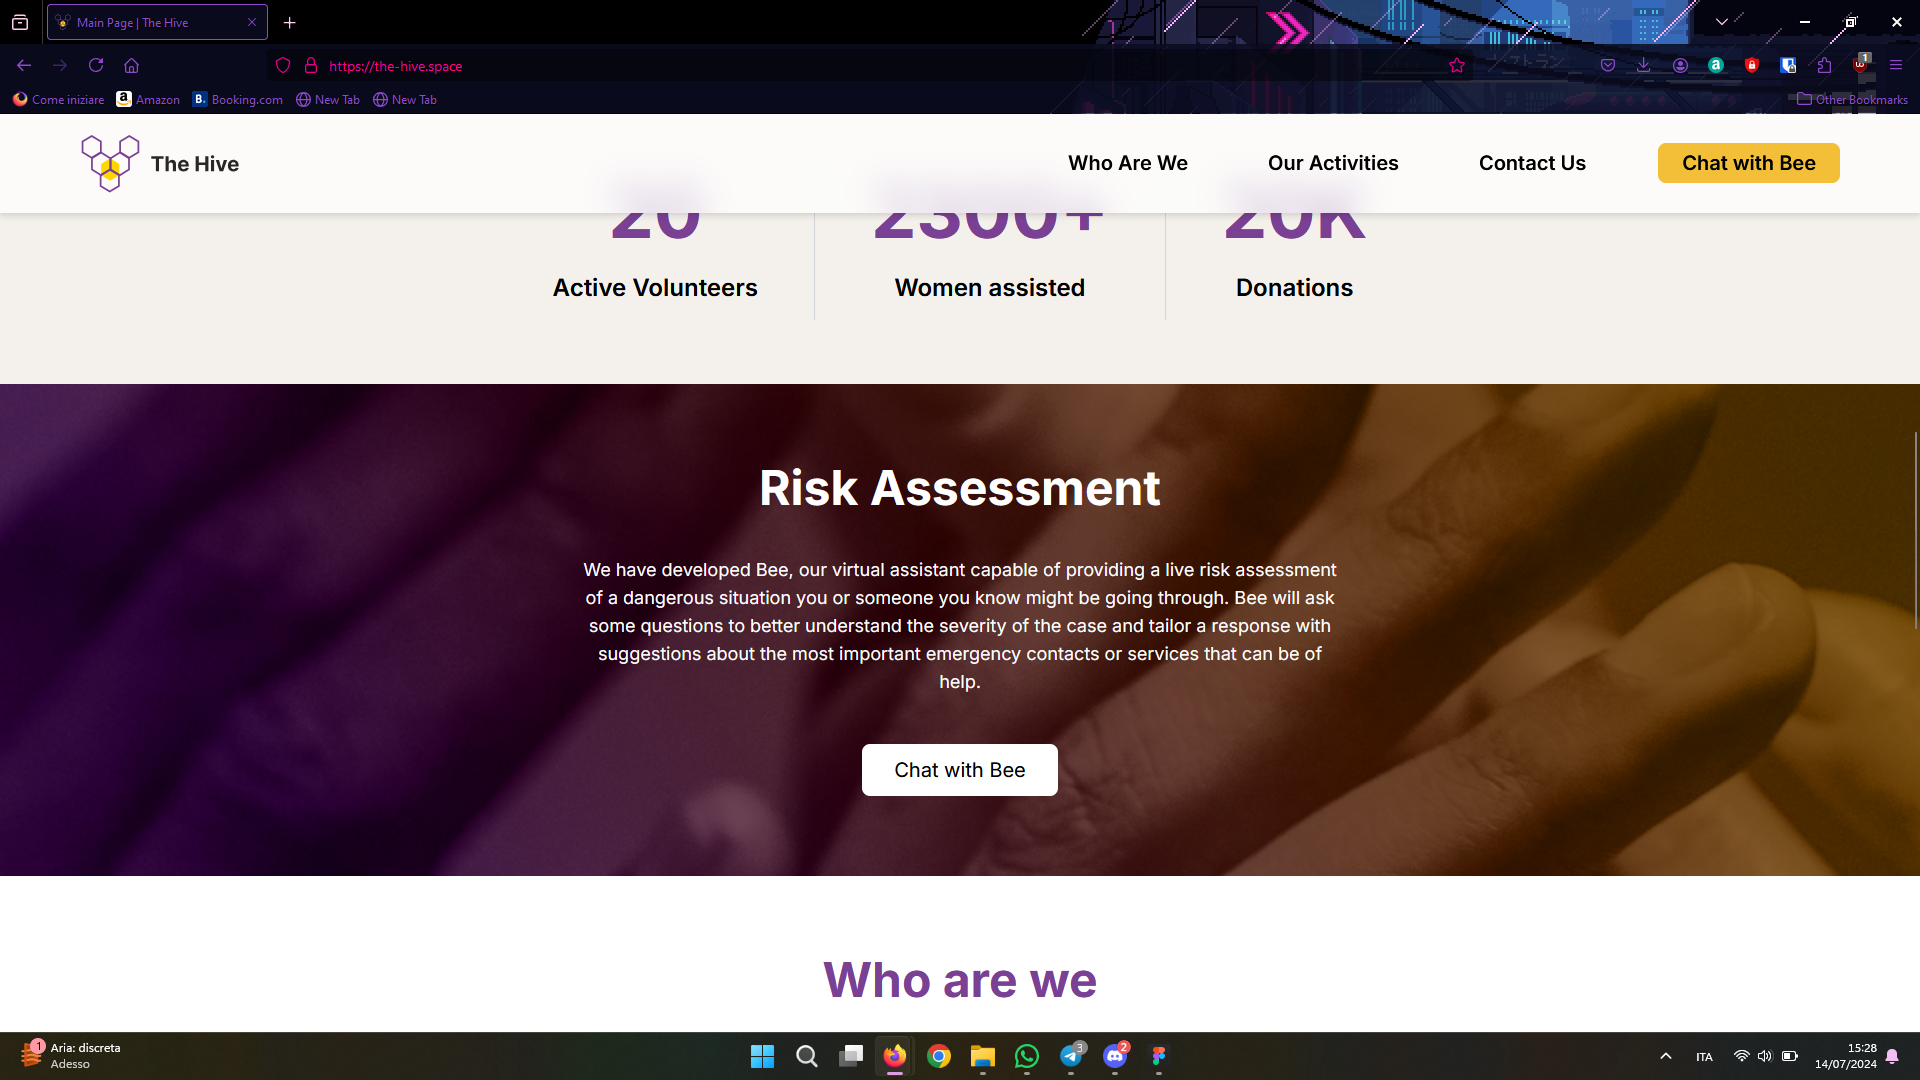
\includegraphics[width=0.5\linewidth]{img/design-document/website-screenshots/homepage-3.png}
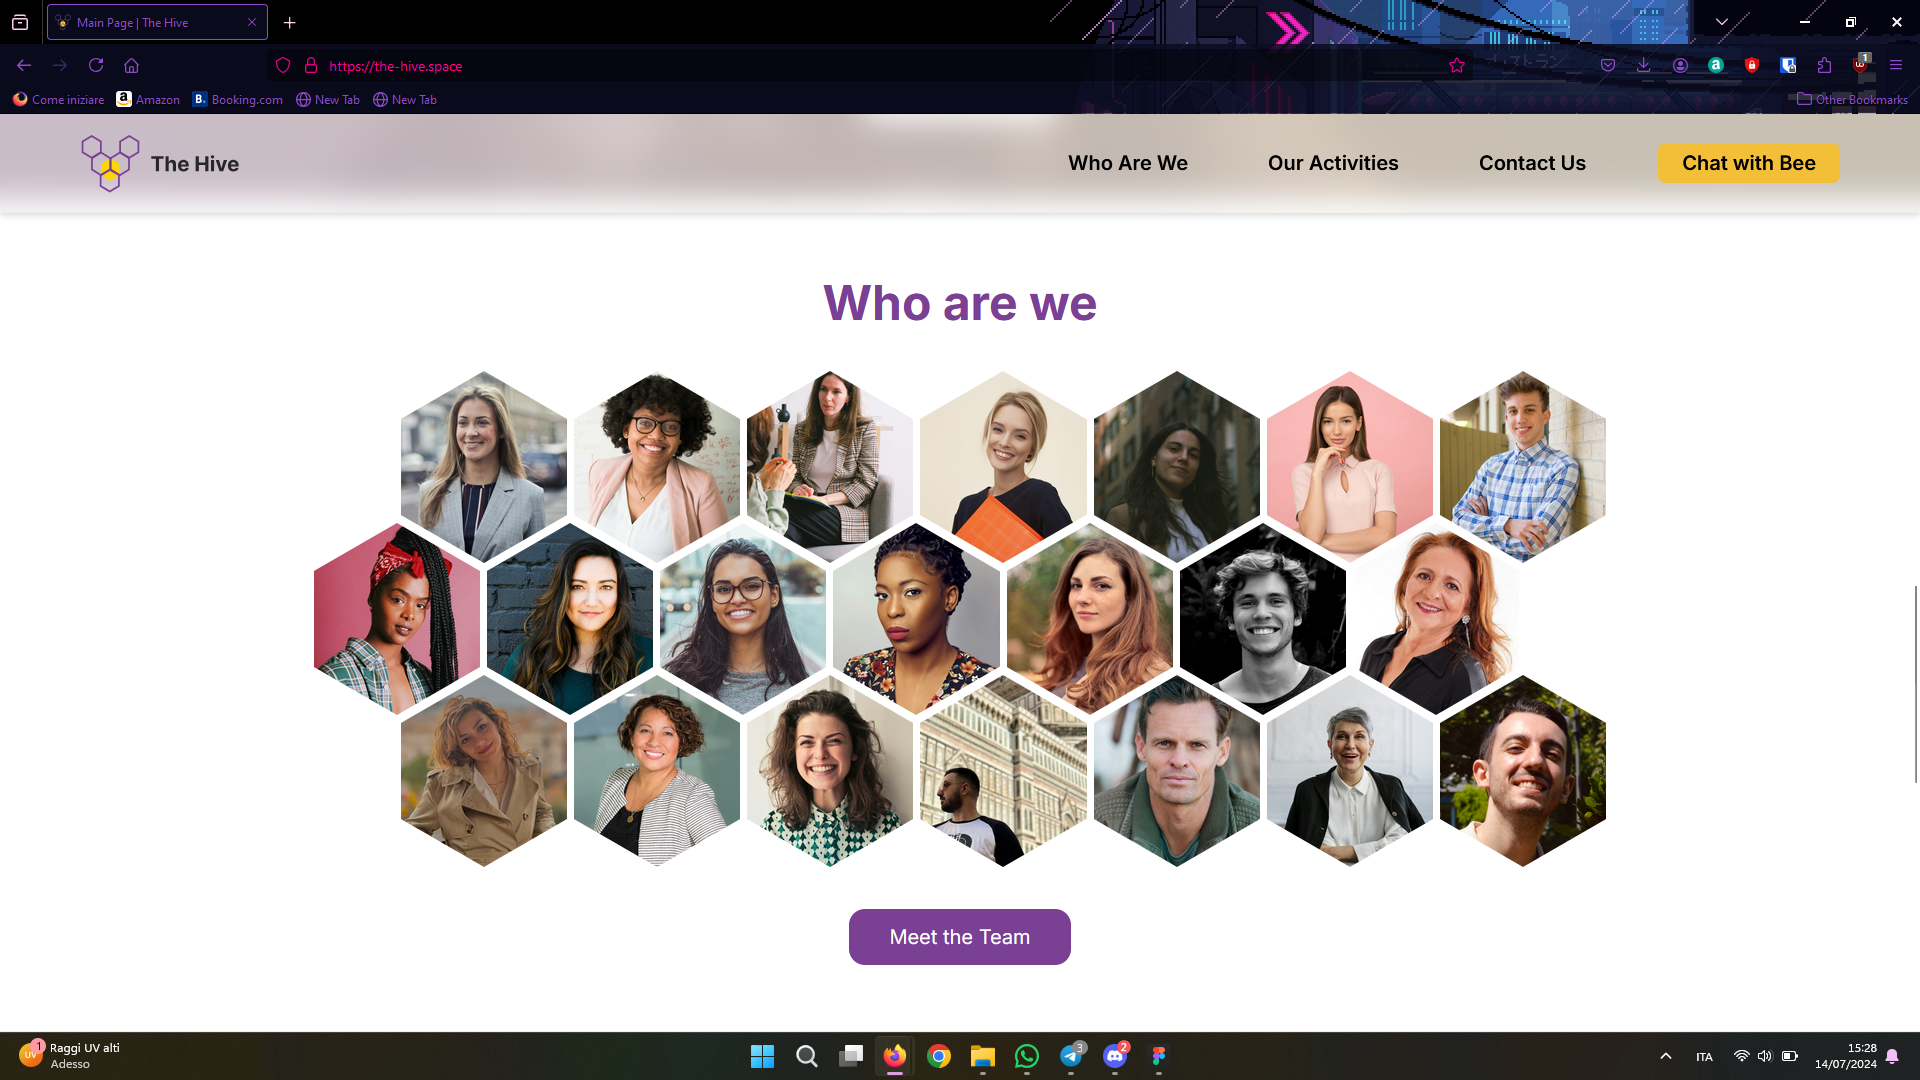
\includegraphics[width=0.5\linewidth]{img/design-document/website-screenshots/homepage-4.png}
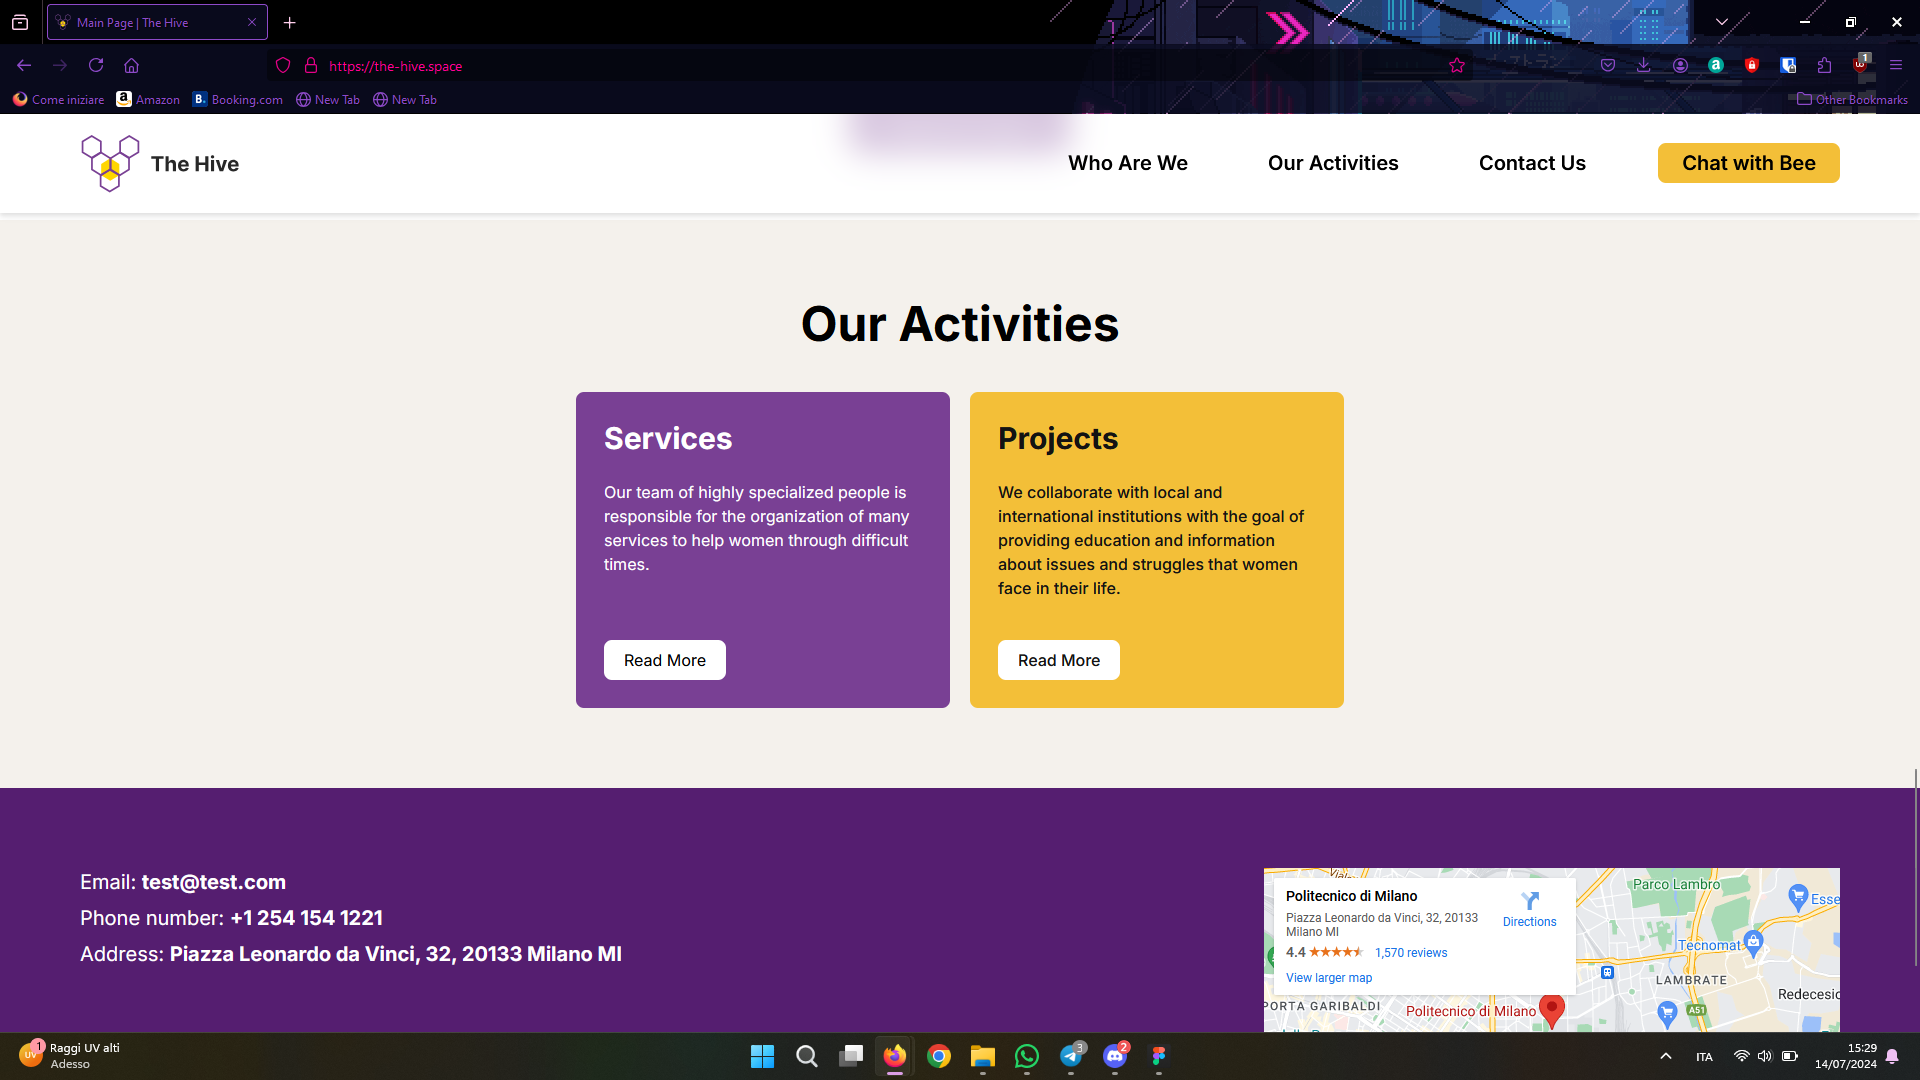
\includegraphics[width=0.5\linewidth]{img/design-document/website-screenshots/homepage-5.png}

%About The Center
\subsection{The Center}
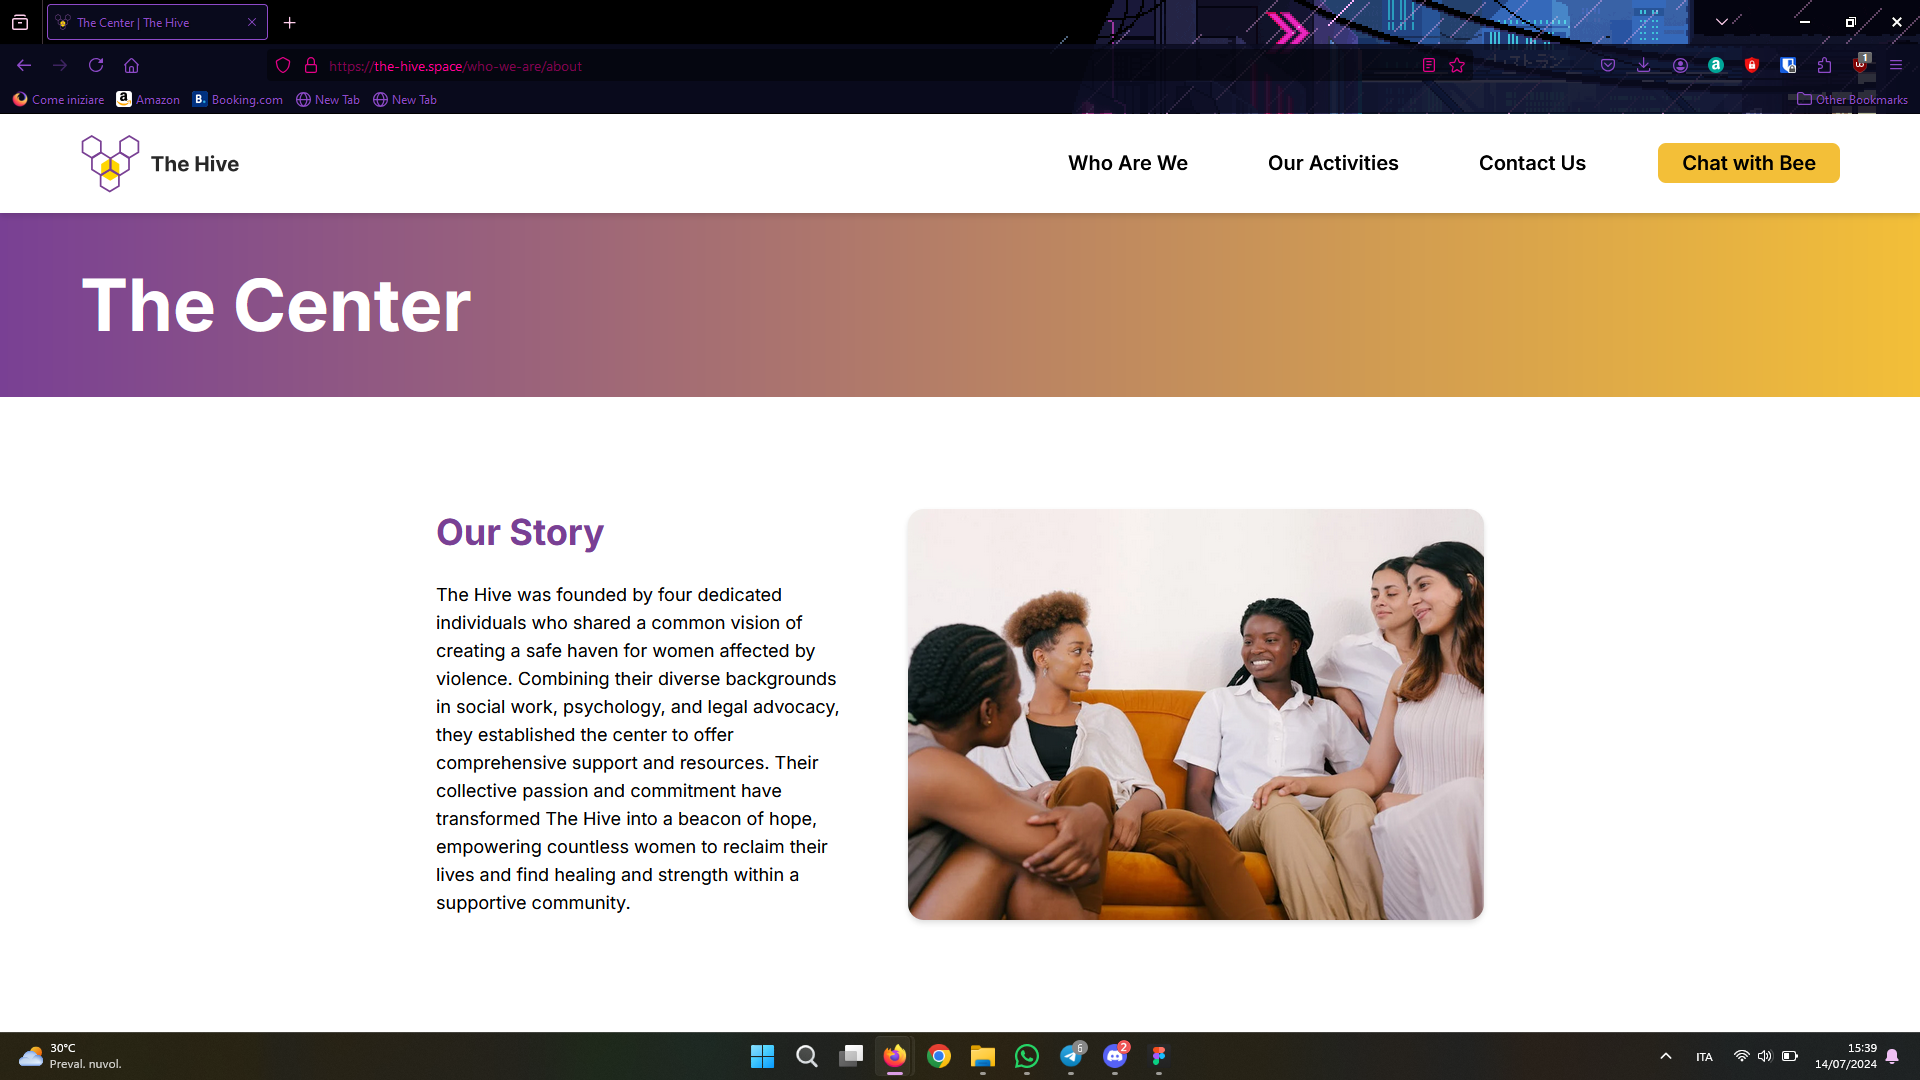
\includegraphics[width=0.5\linewidth]{img/design-document/website-screenshots/centerpage.png}

%Our Team + Single Person
\subsection{Our Team}
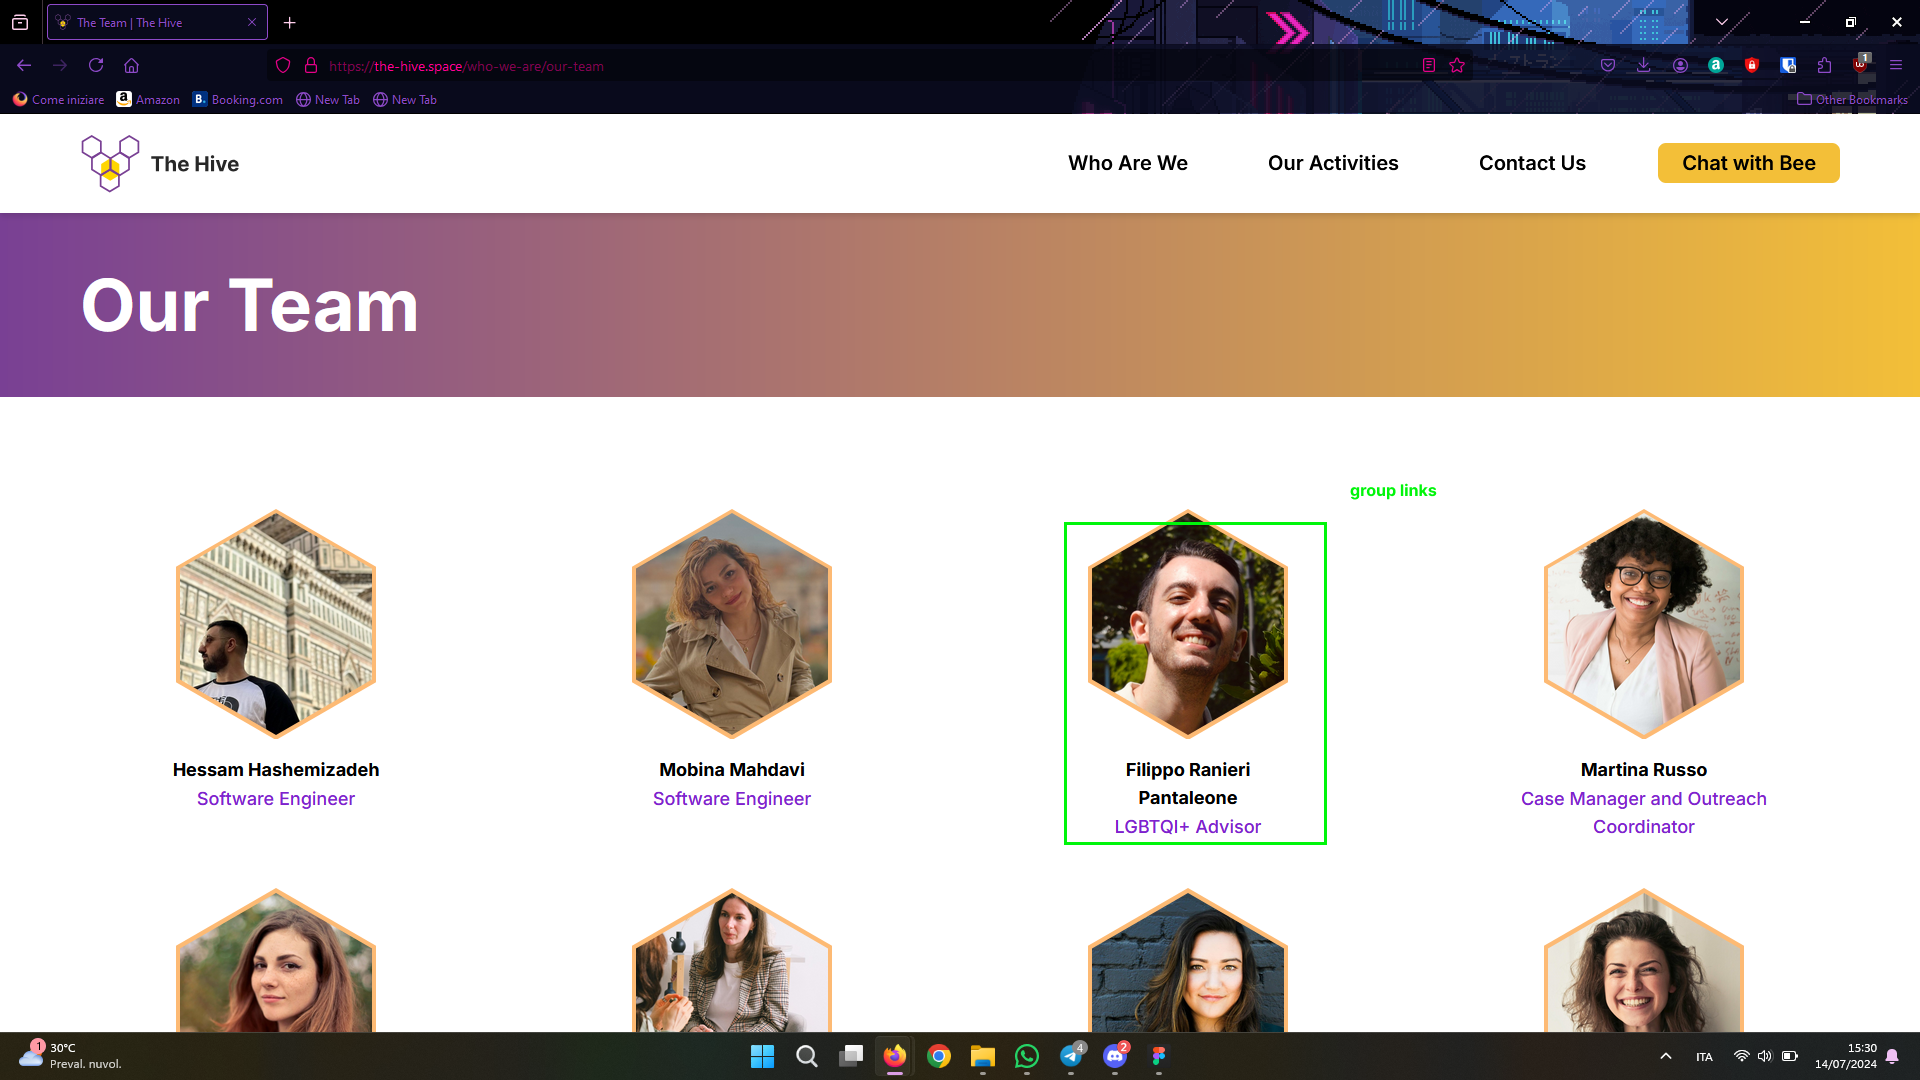
\includegraphics[width=0.5\linewidth]{img/design-document/website-screenshots/teampage.png}
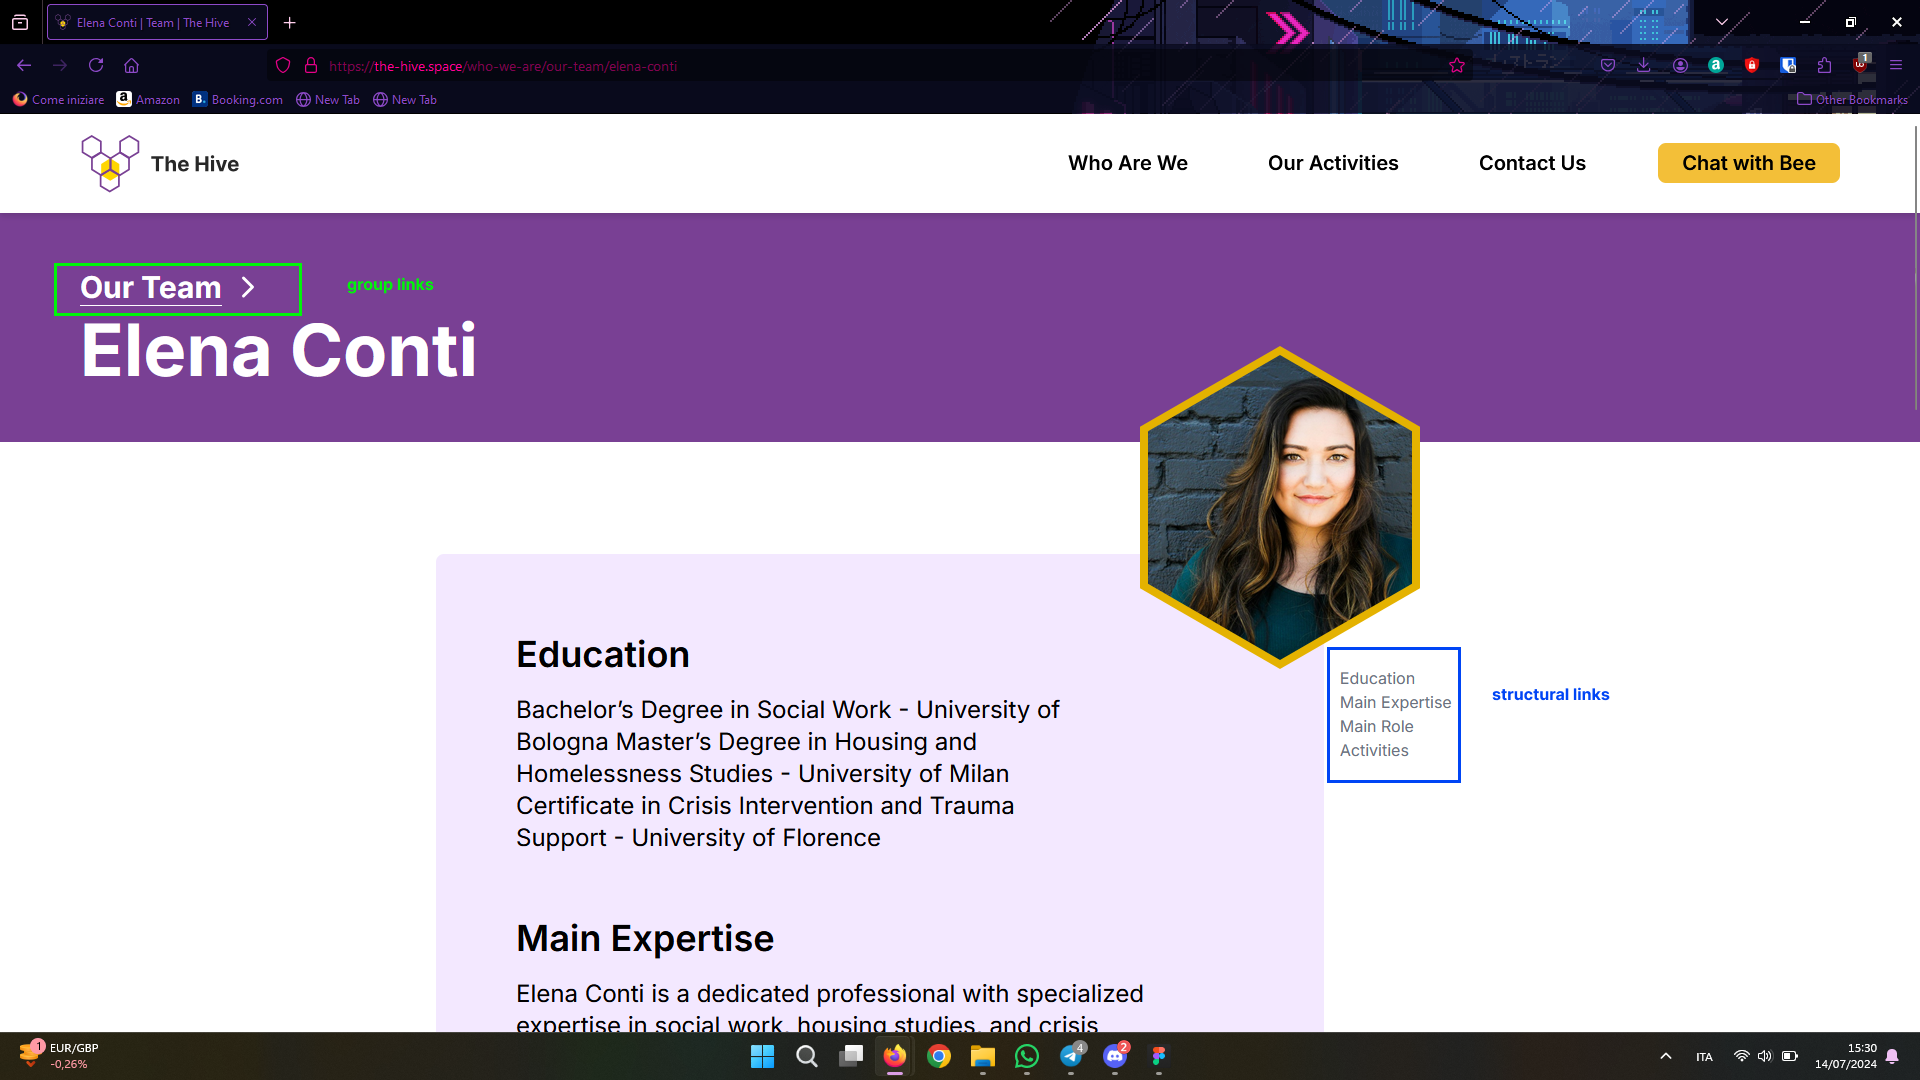
\includegraphics[width=0.5\linewidth]{img/design-document/website-screenshots/personpage-1.png}
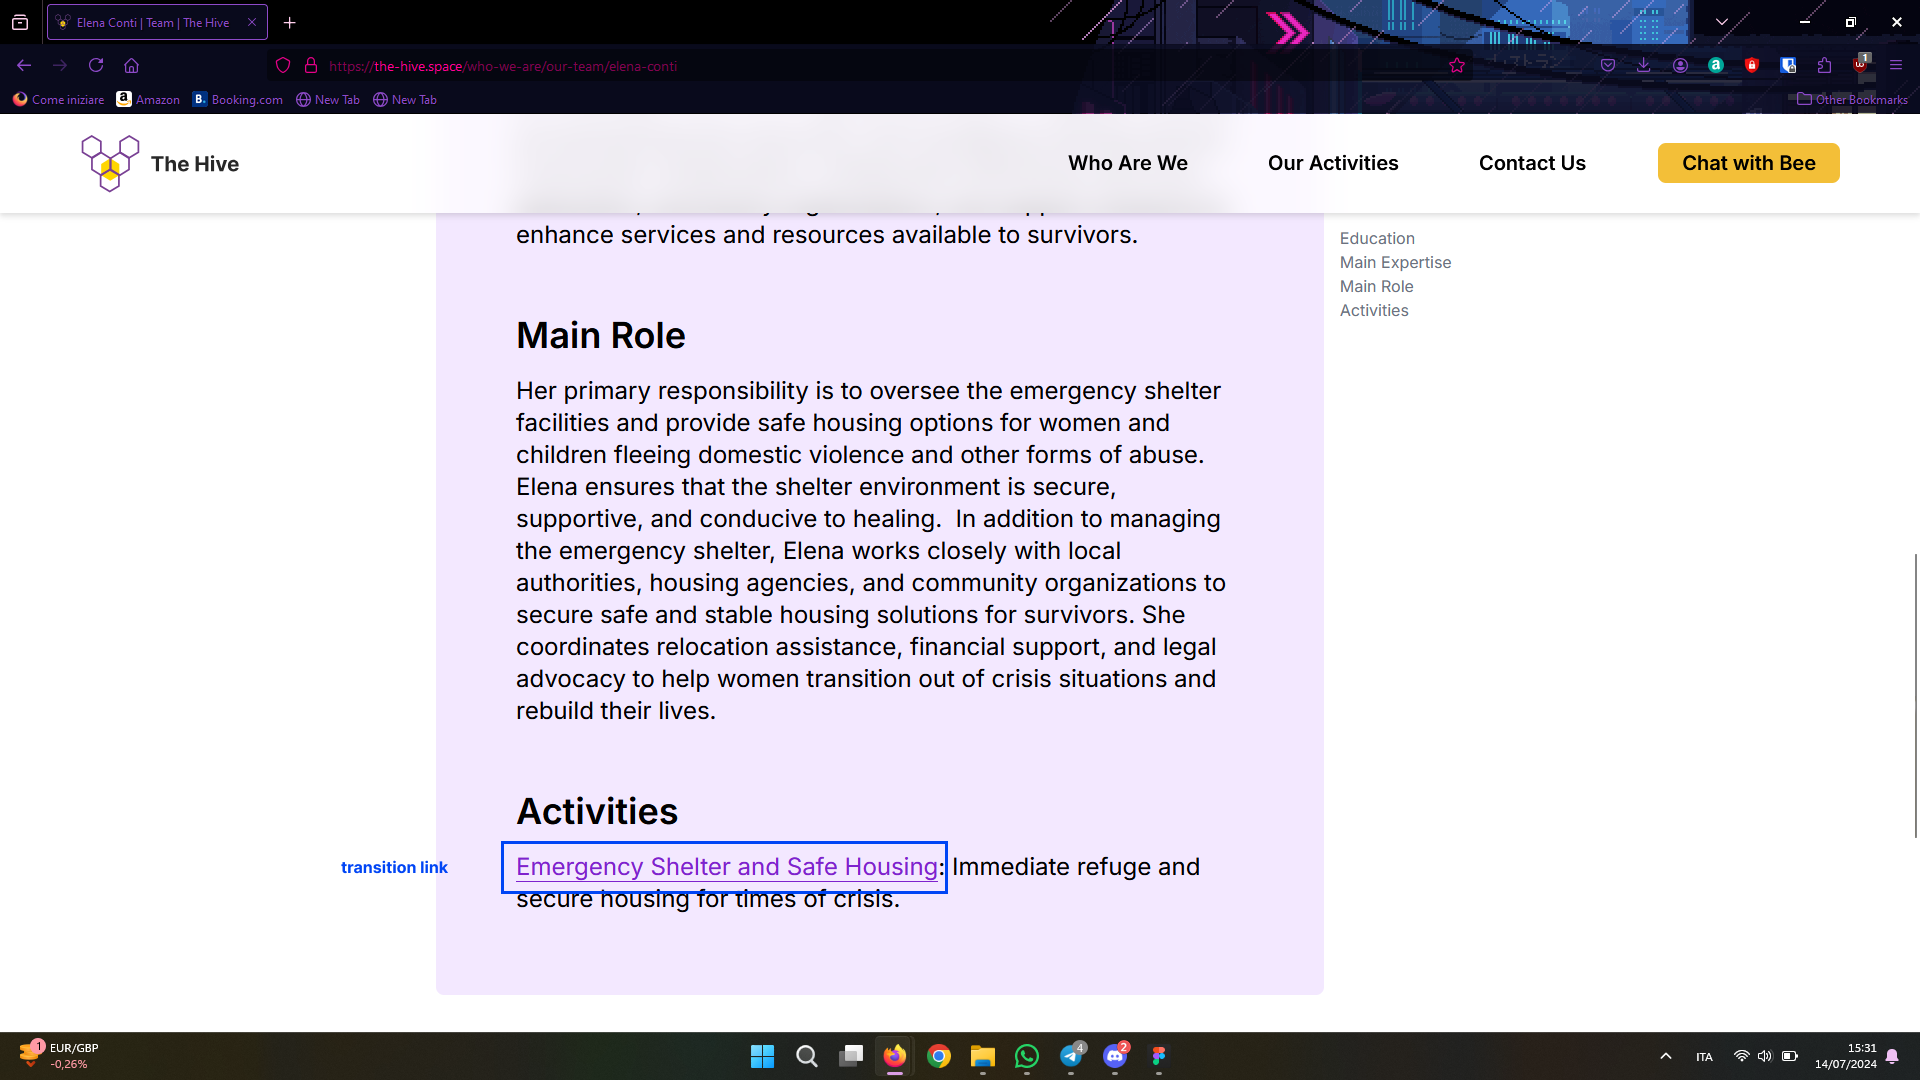
\includegraphics[width=0.5\linewidth]{img/design-document/website-screenshots/personpage-2.png}

%Our Services + Single Service
\subsection{Services}
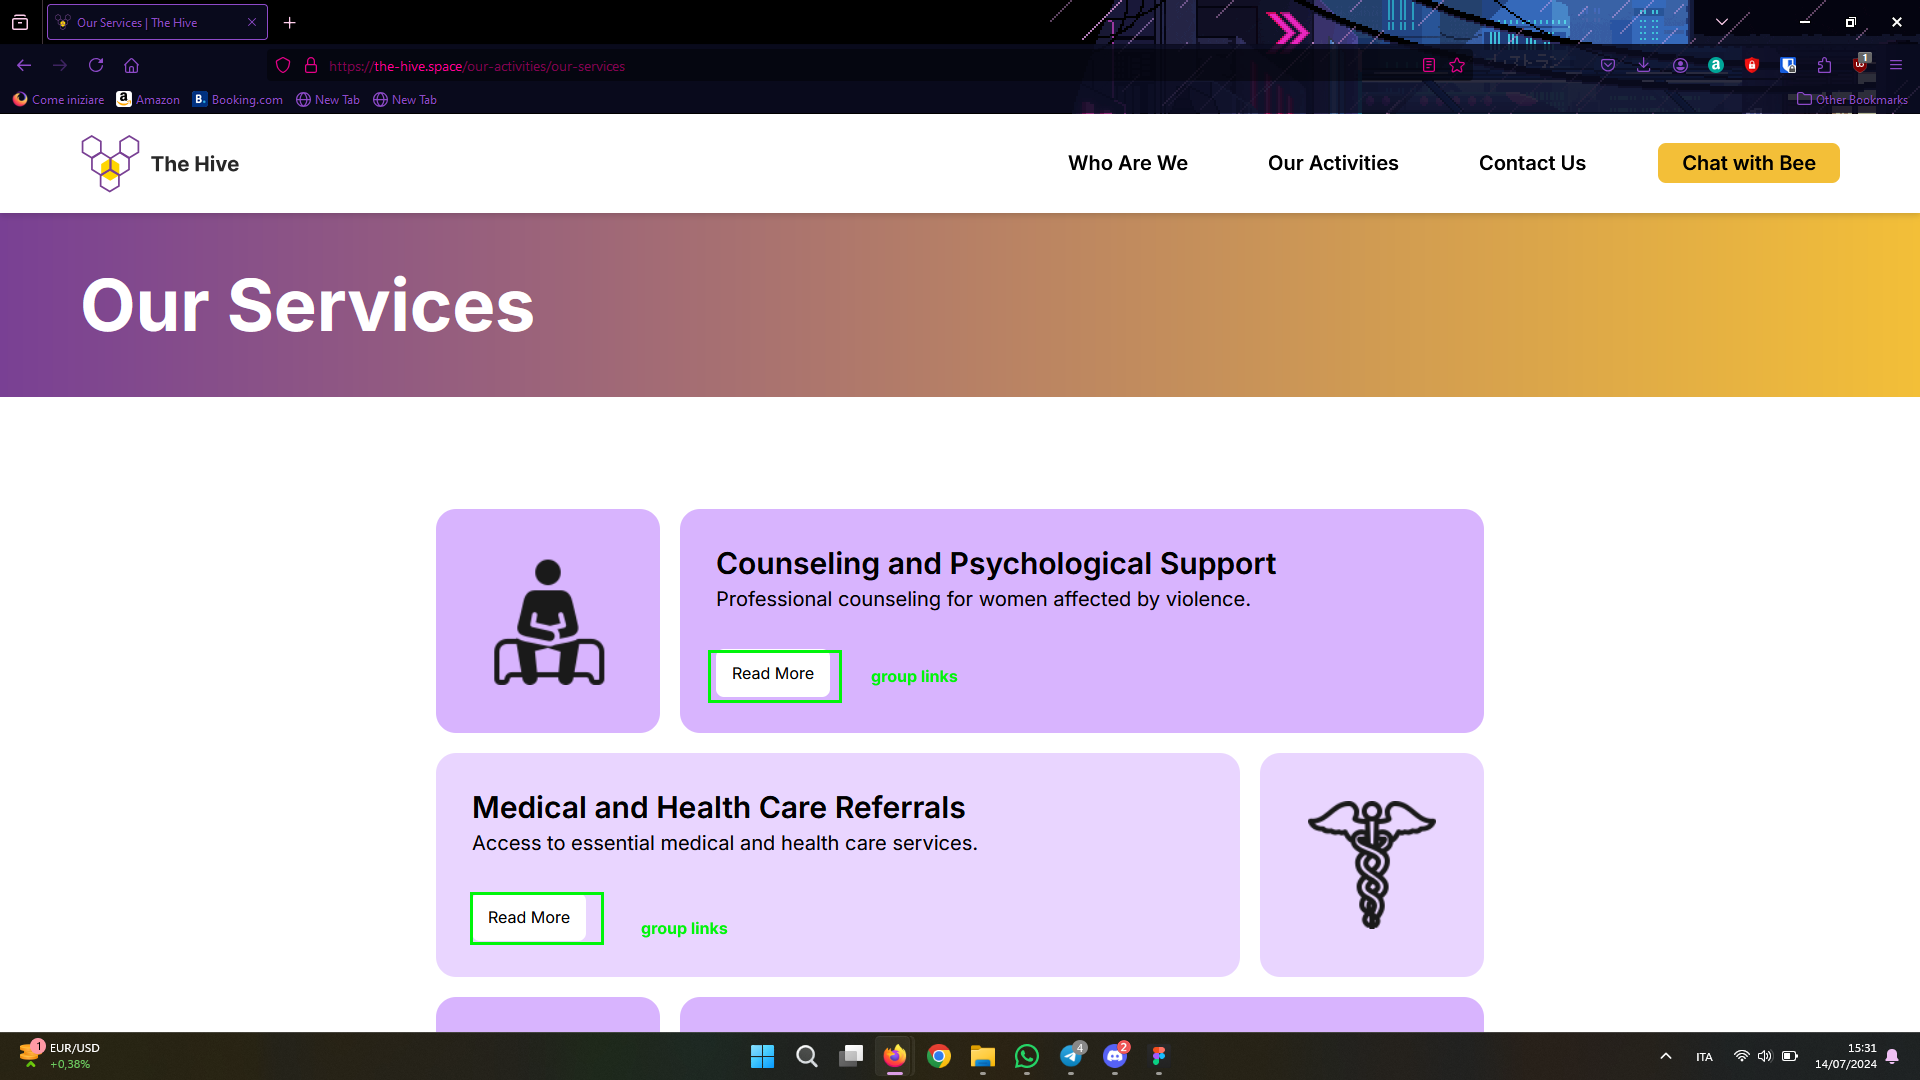
\includegraphics[width=0.5\linewidth]{img/design-document/website-screenshots/servicespage.png}
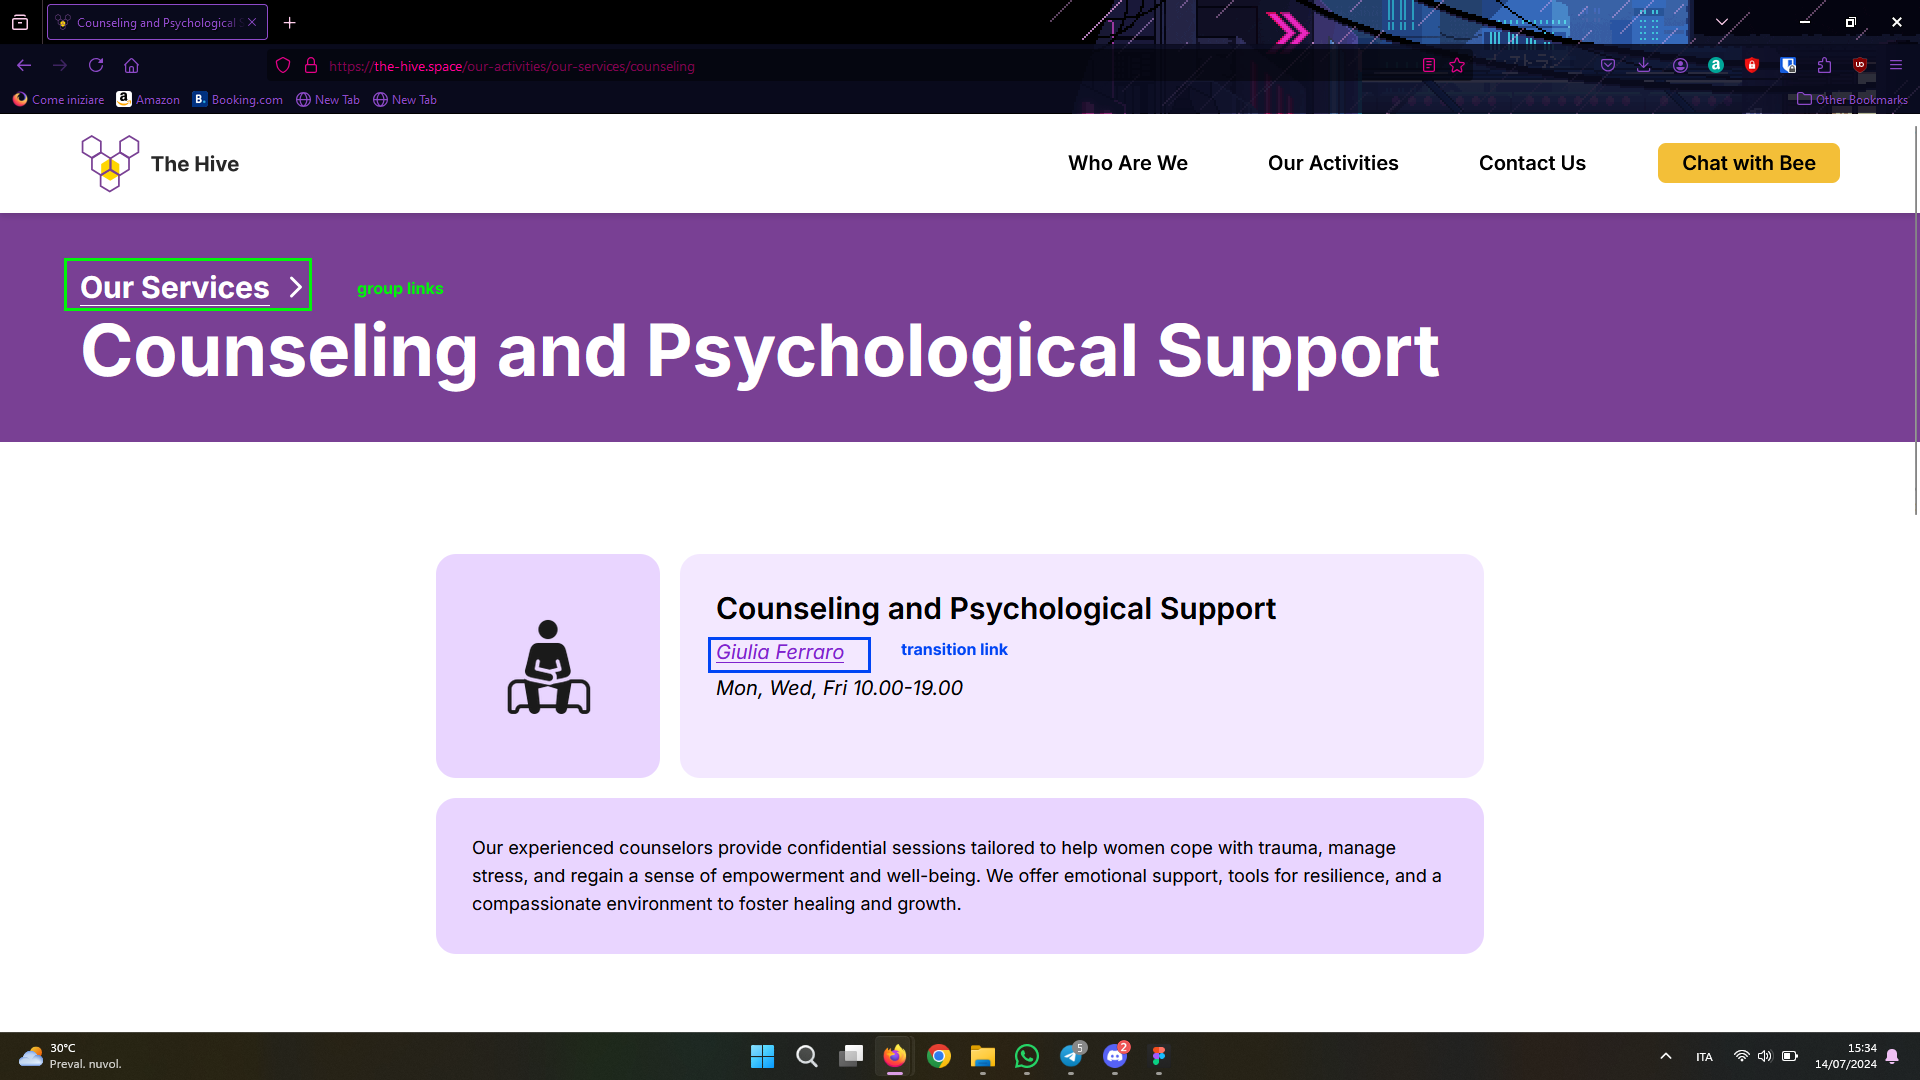
\includegraphics[width=0.5\linewidth]{img/design-document/website-screenshots/servicepage-1.png}
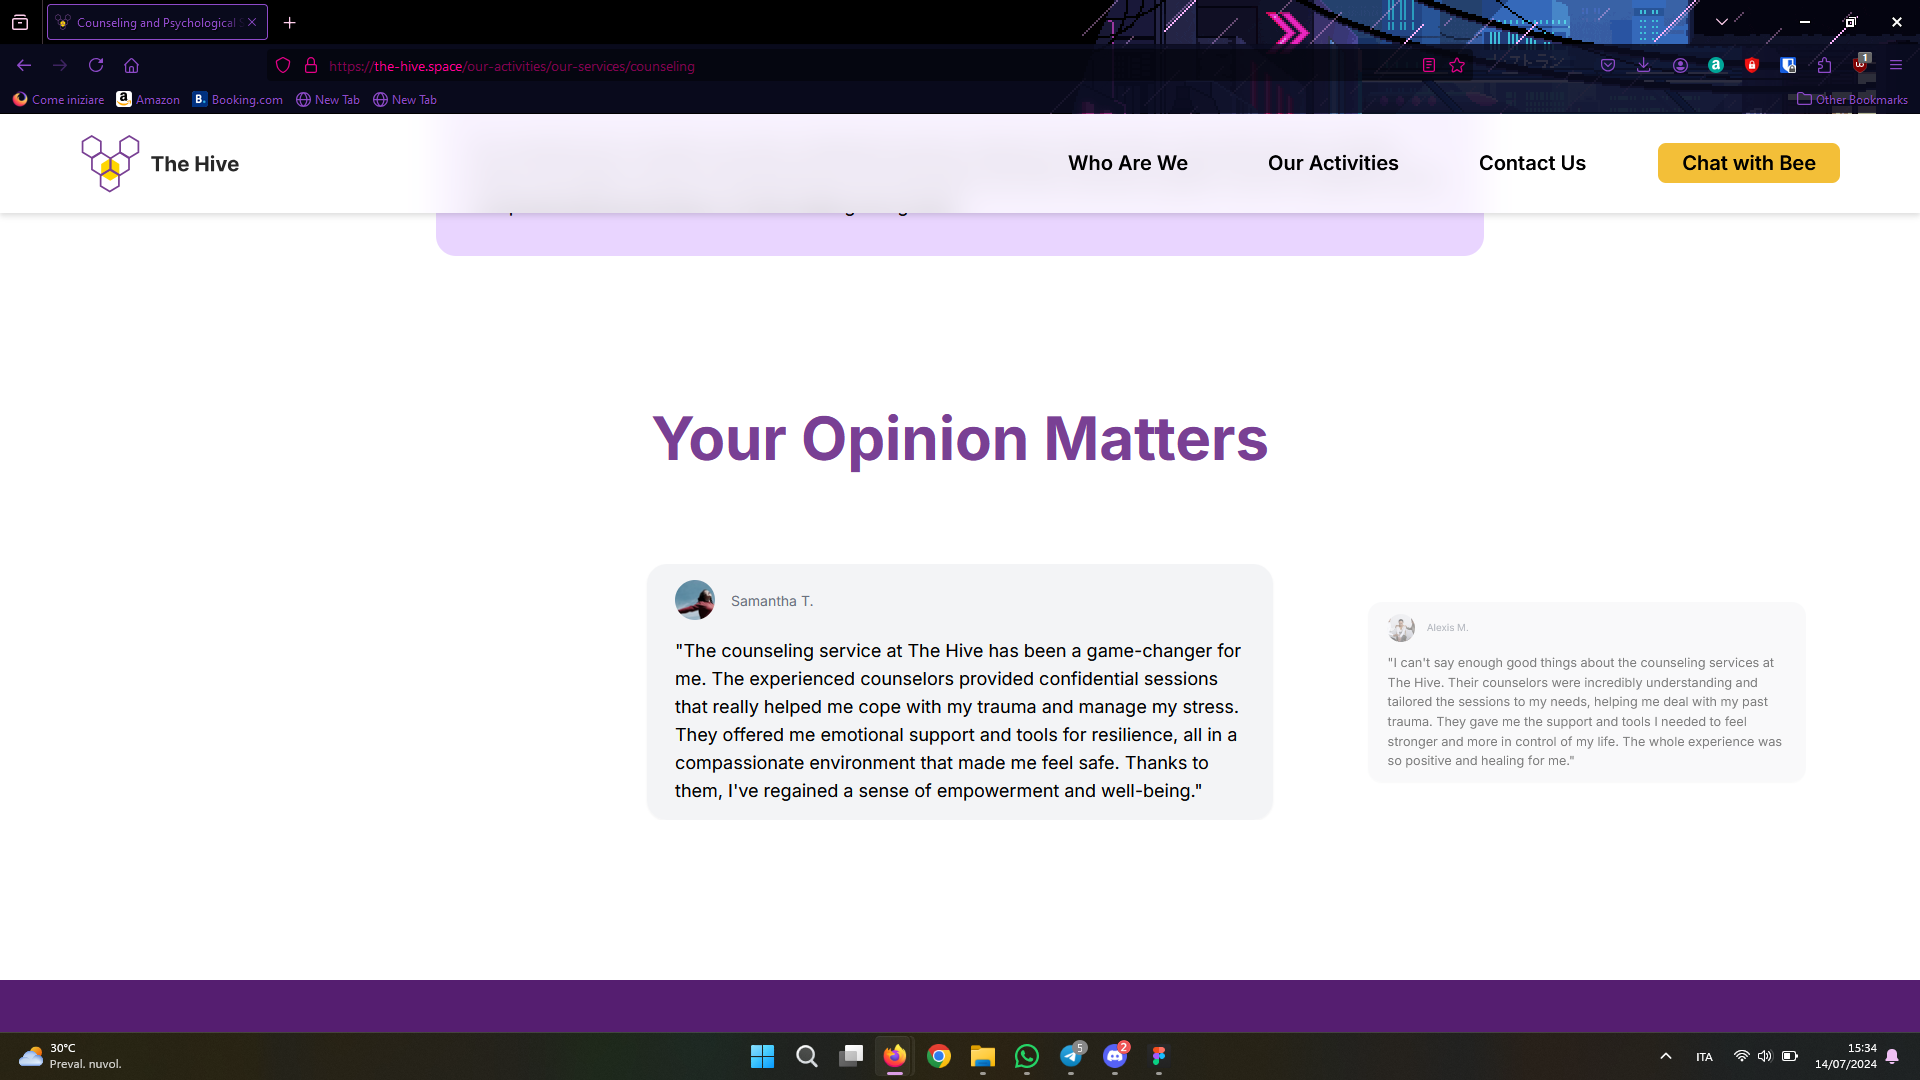
\includegraphics[width=0.5\linewidth]{img/design-document/website-screenshots/servicepage-2.png}

%Our Projects + Single Project
\subsection{Our Projects}
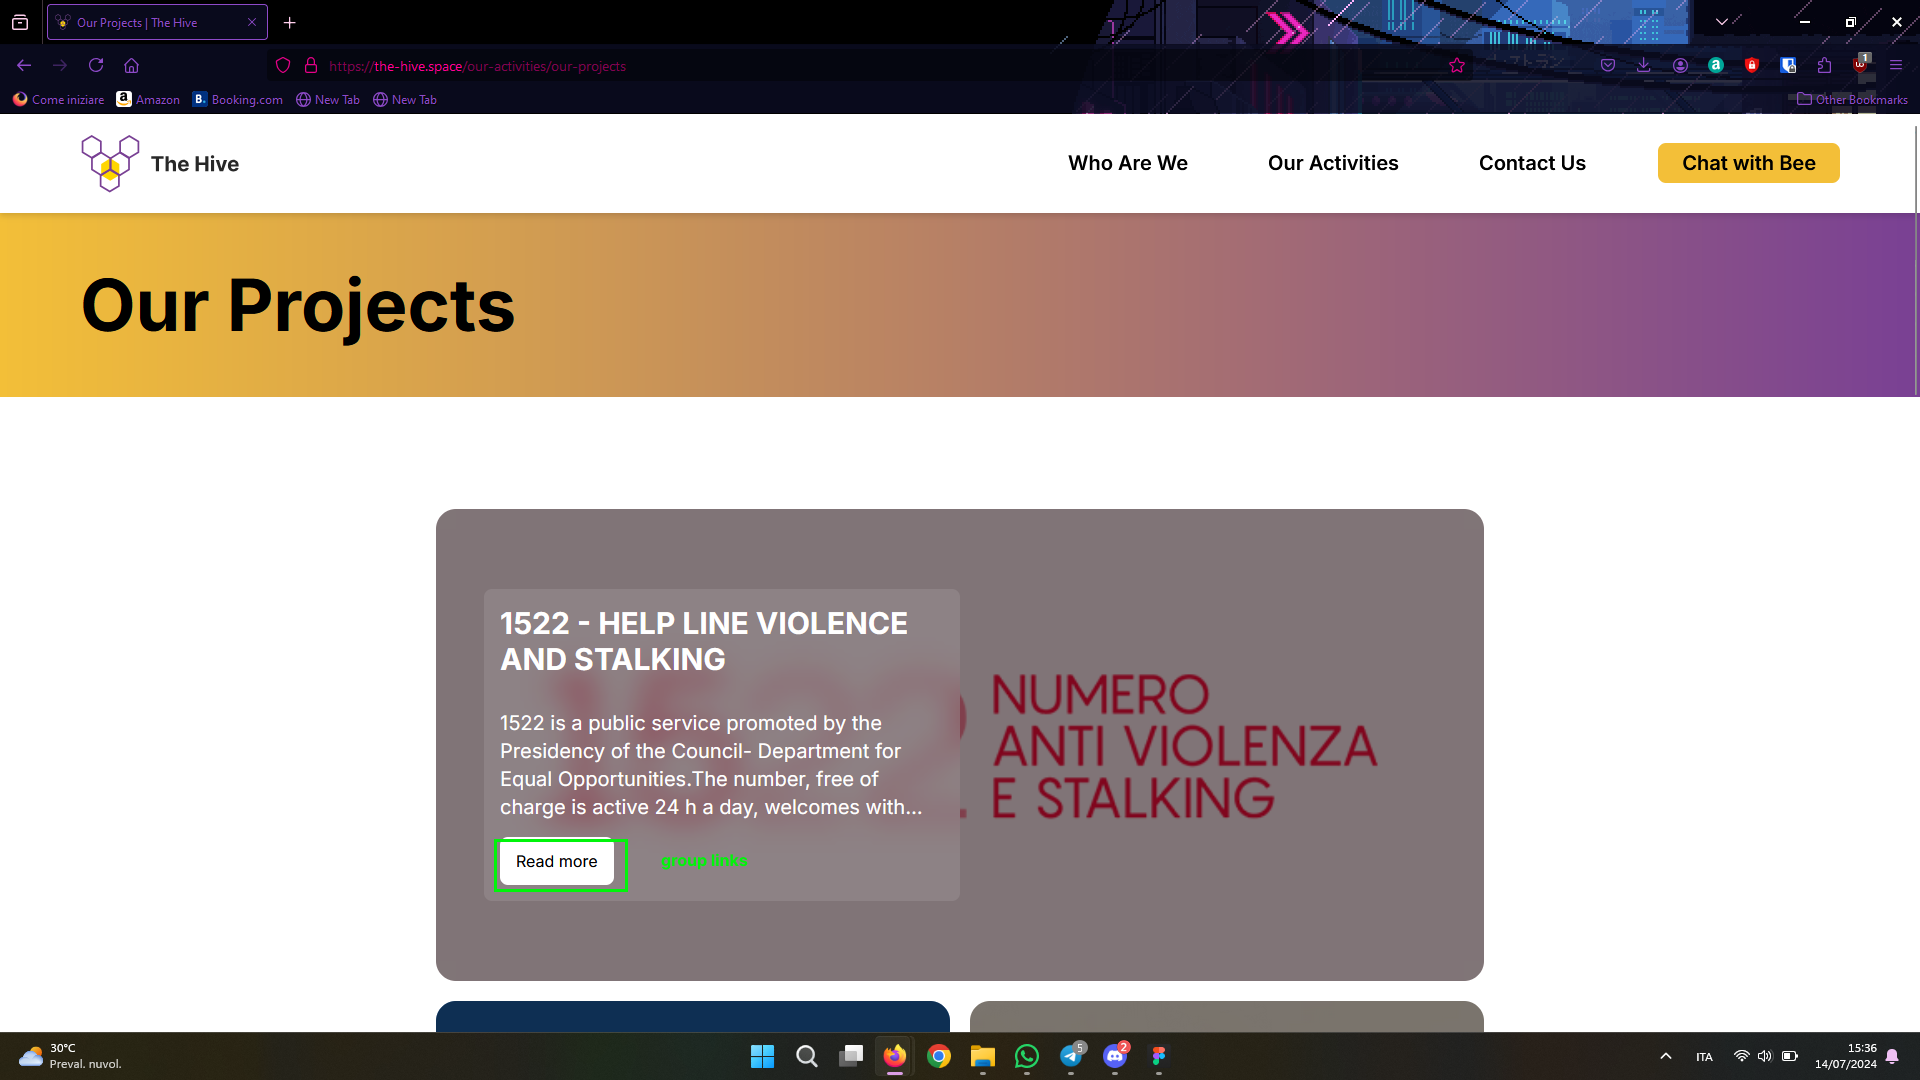
\includegraphics[width=0.5\linewidth]{img/design-document/website-screenshots/projectspage.png}
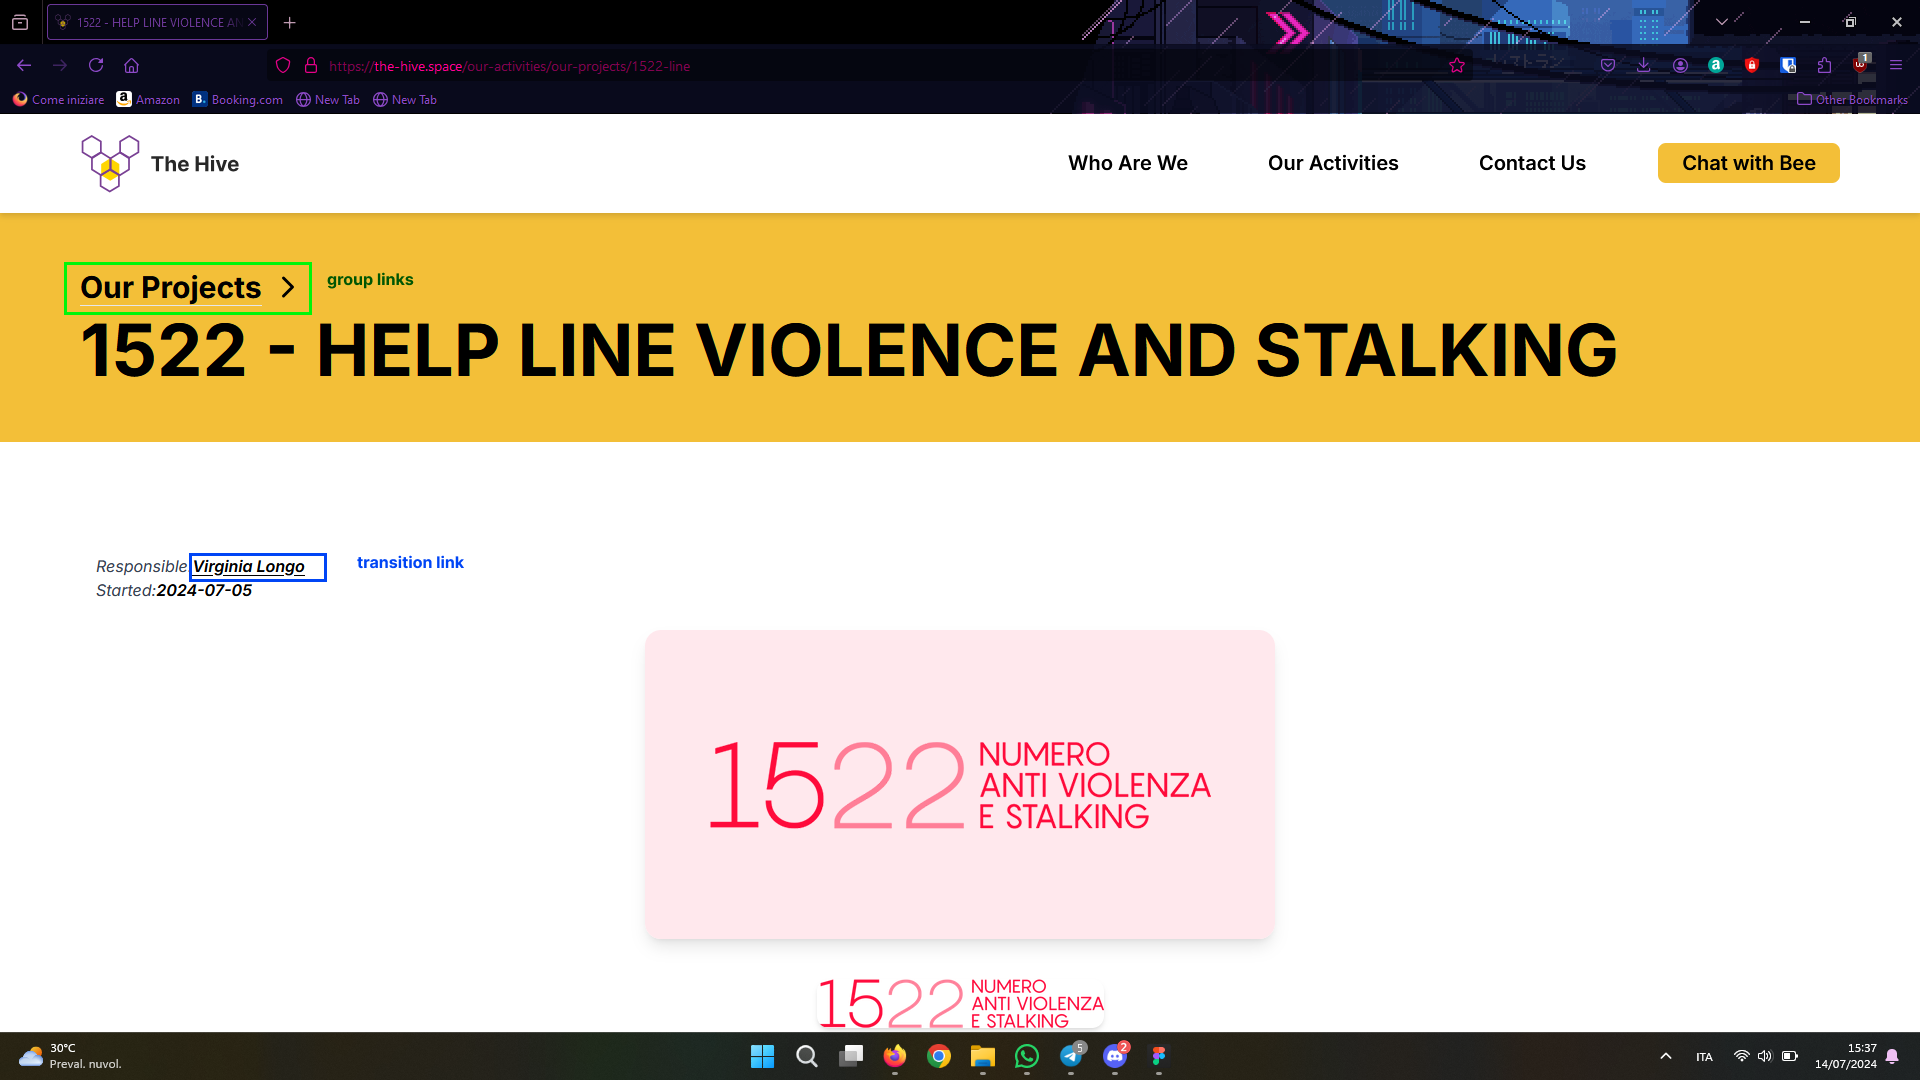
\includegraphics[width=0.5\linewidth]{img/design-document/website-screenshots/projectpage-1.png}

%Contacts
\subsection{Contacts}
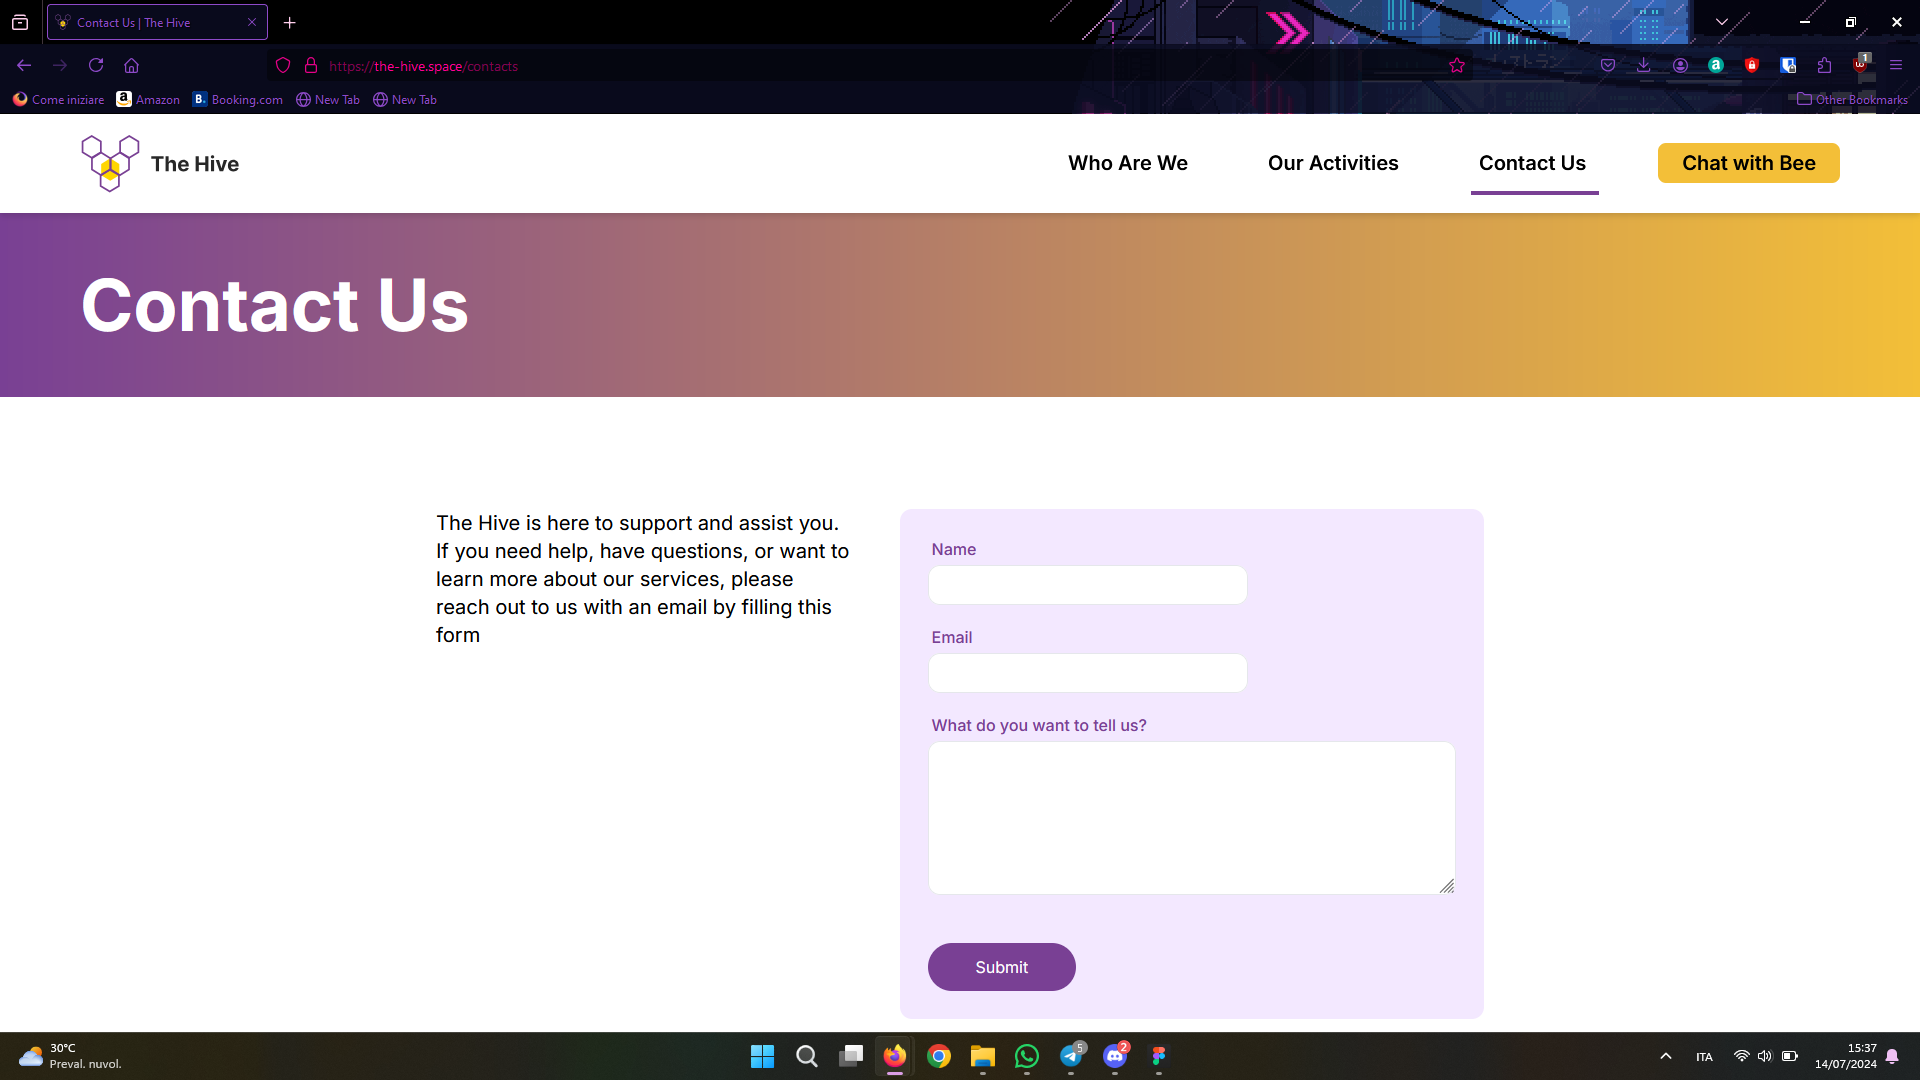
\includegraphics[width=0.5\linewidth]{img/design-document/website-screenshots/contacts.png}

%Chatbot
\subsection{Chatbot}
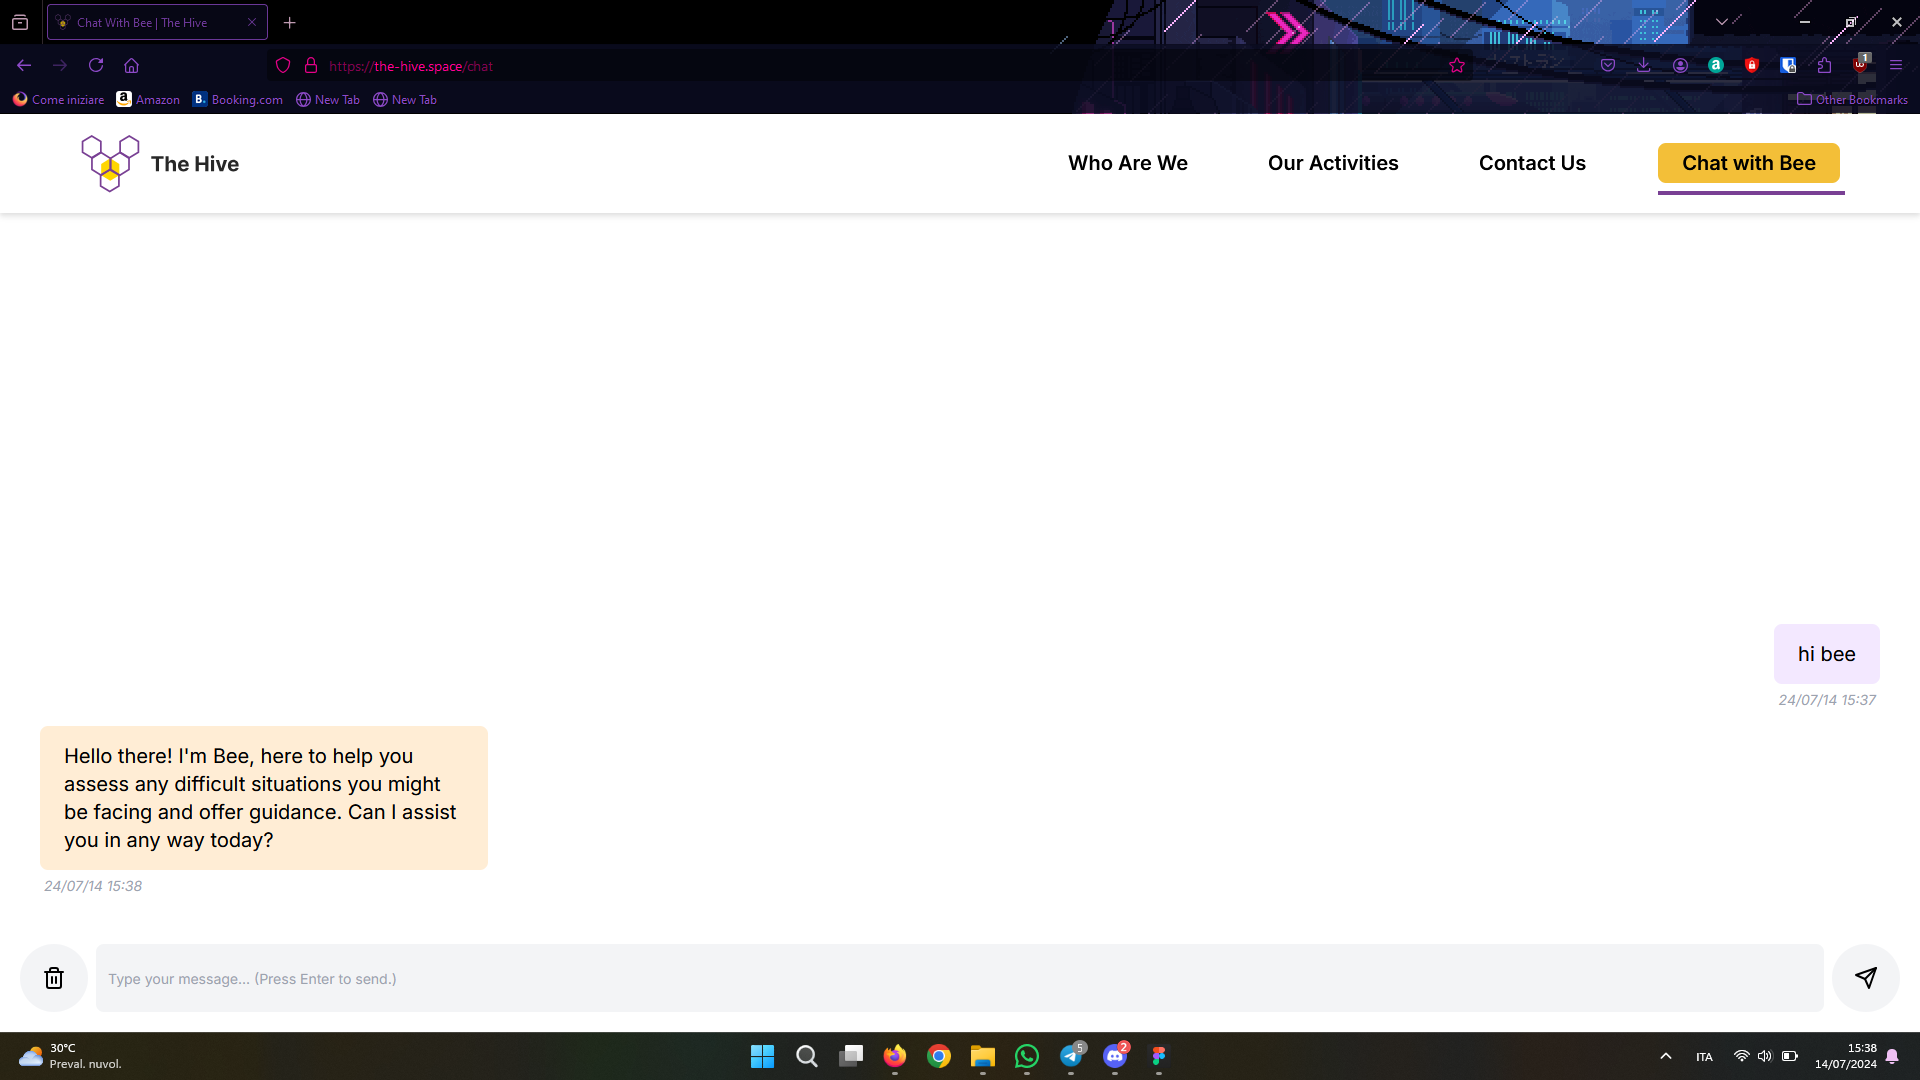
\includegraphics[width=0.5\linewidth]{img/design-document/website-screenshots/chatbot.png}


\pagebreak
\section{Interaction Scenarios}
%Description
\subsection{Scenario 1}
Alessia M. is a 32 year old woman that has recently came out of an abusive relationship with her boyfriend of 7 years.
She knows that her healing process is going to take a long time and that she will need help through it.
A friend suggests her to check out The Hive, and mentions to her that the Center offers a psychological counseling service
that could help her. She starts by checking out the website: scrolling through the homepage she finds a link to the about page
of The Hive and reads through to get an idea of what the center is about. Satisfied with what she reads she uses the navigation
bar (landmarks) to find the service her friend talked to her about. Sure enough in the list of services there is the “Counseling
and Psychological Support”, she navigates to the single Service Page through the “Read More” (group link) and reads through the
additional information and testimonials, and decides to give it a try next Friday.

%Screenshots
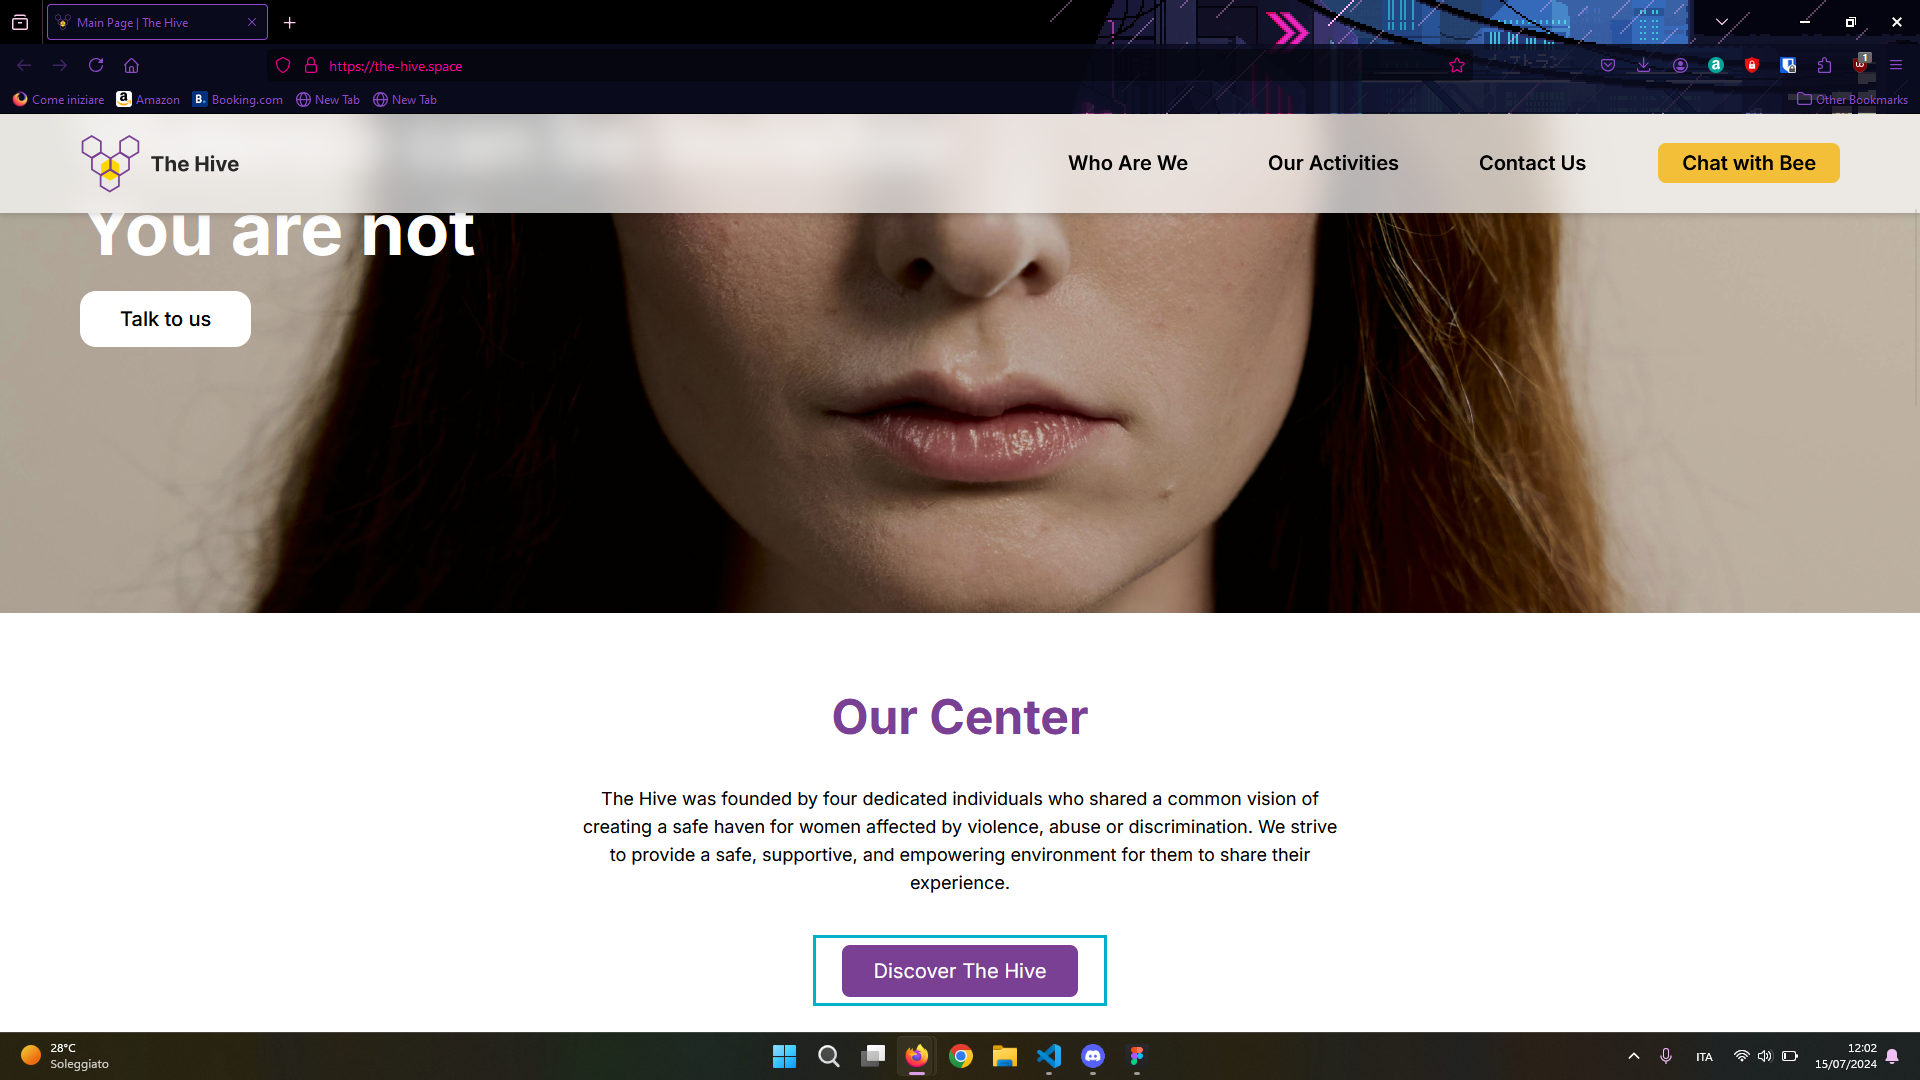
\includegraphics[width=0.5\linewidth]{img/design-document/interaction-scenarios/scenario1/step-1.png}
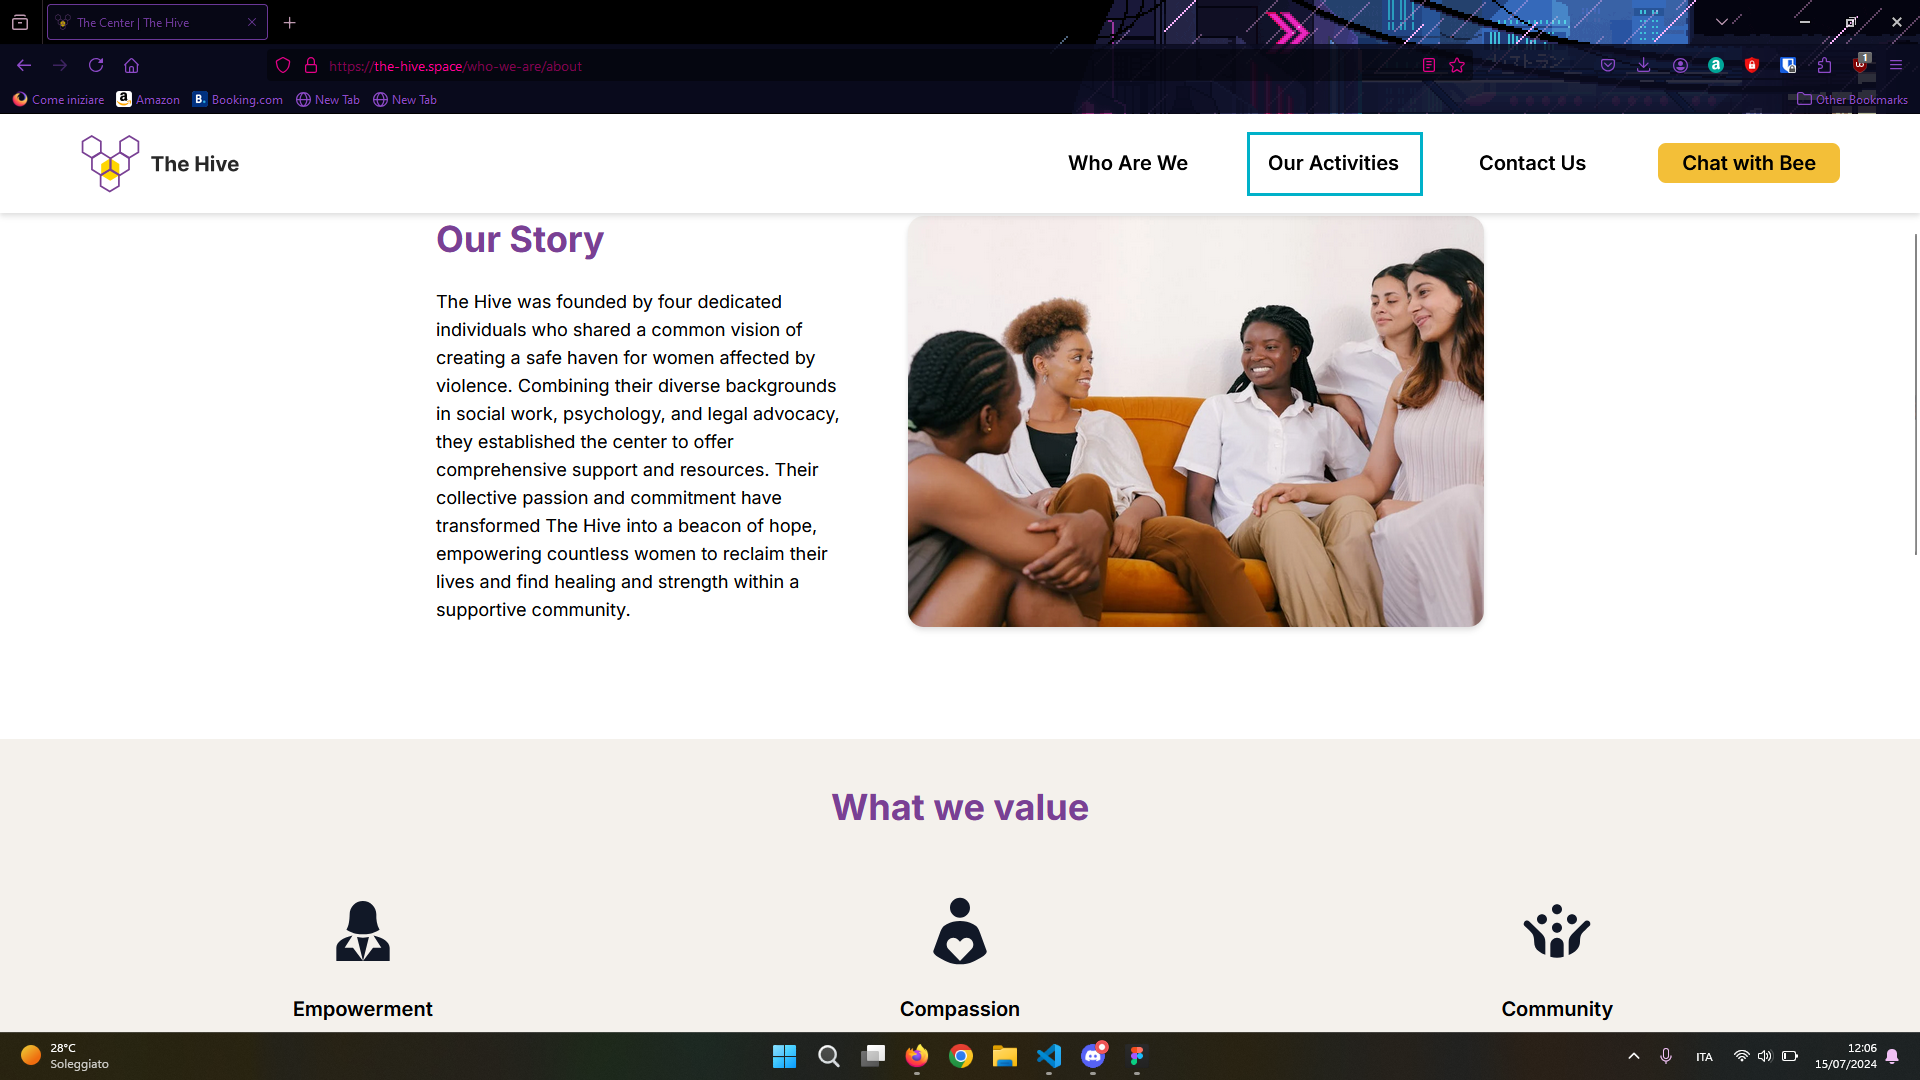
\includegraphics[width=0.5\linewidth]{img/design-document/interaction-scenarios/scenario1/step-2.png}
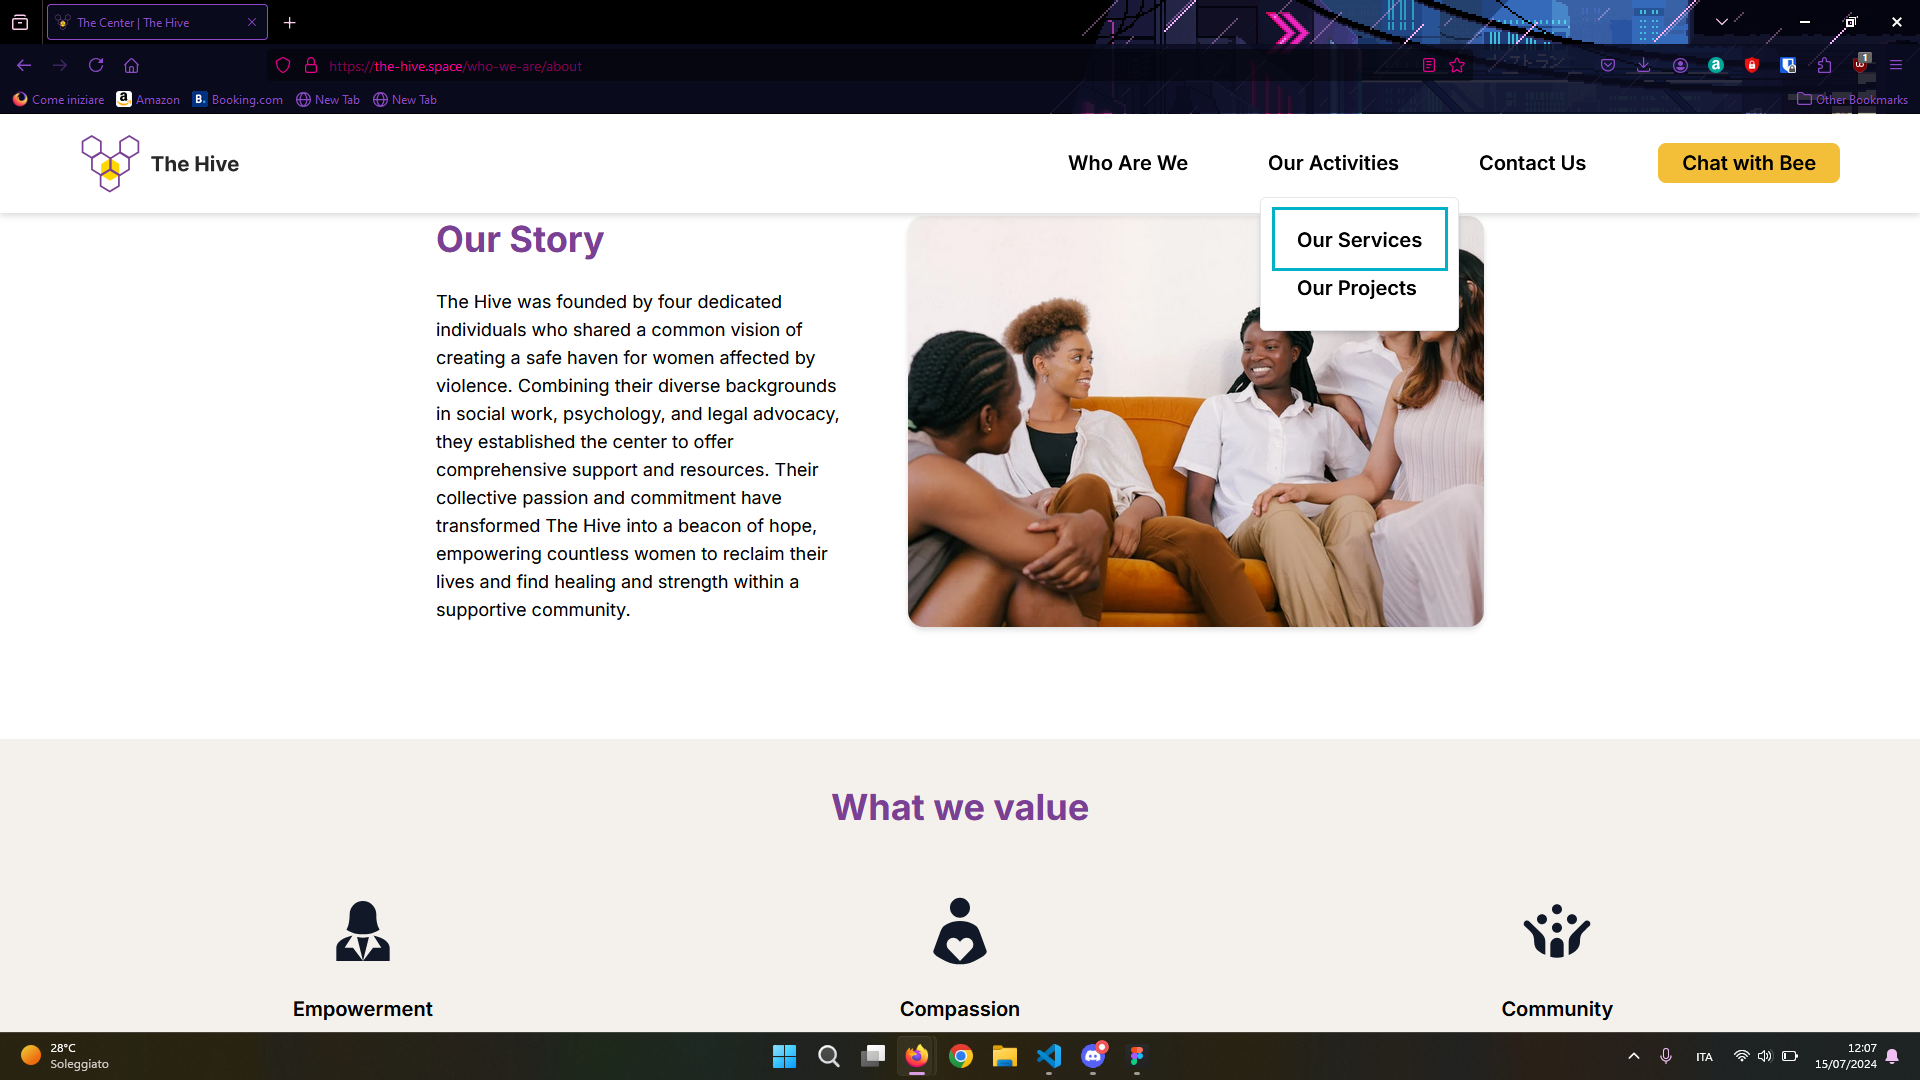
\includegraphics[width=0.5\linewidth]{img/design-document/interaction-scenarios/scenario1/step-3.png}
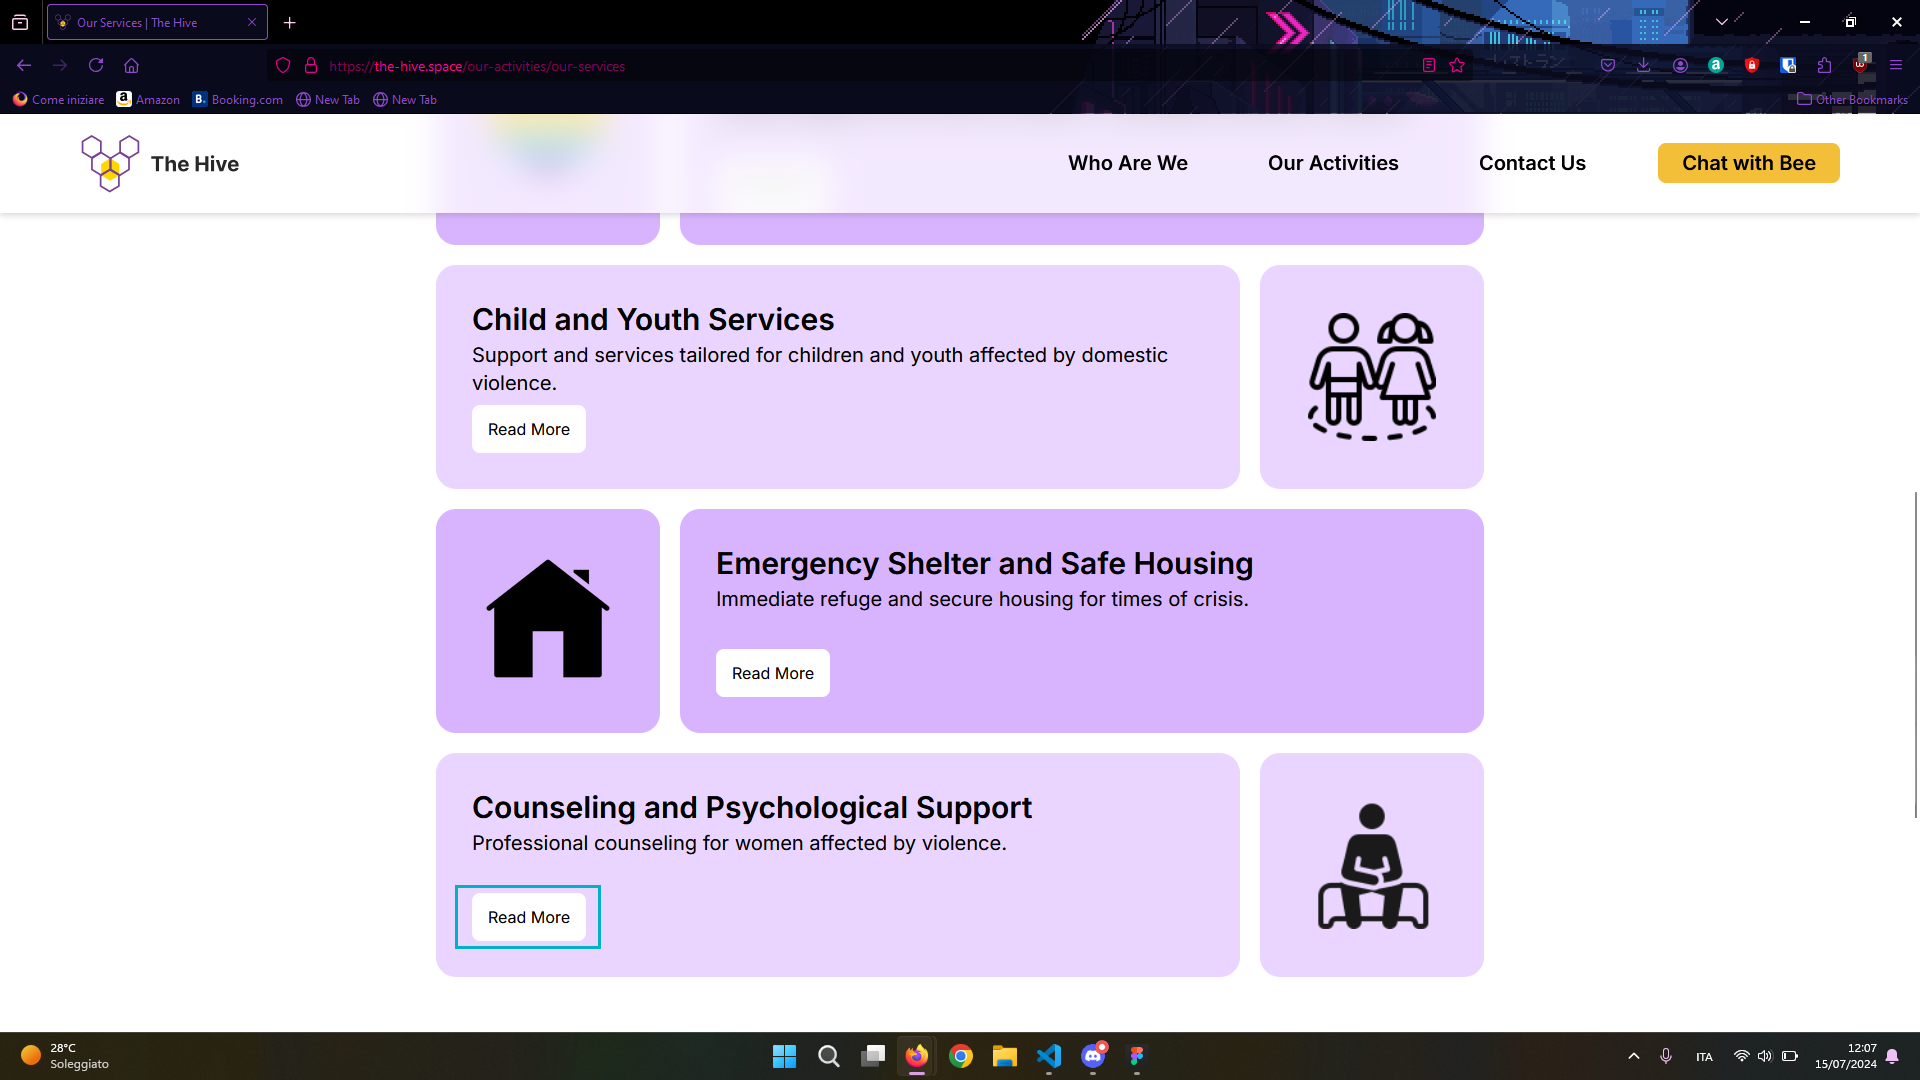
\includegraphics[width=0.5\linewidth]{img/design-document/interaction-scenarios/scenario1/step-4.png}
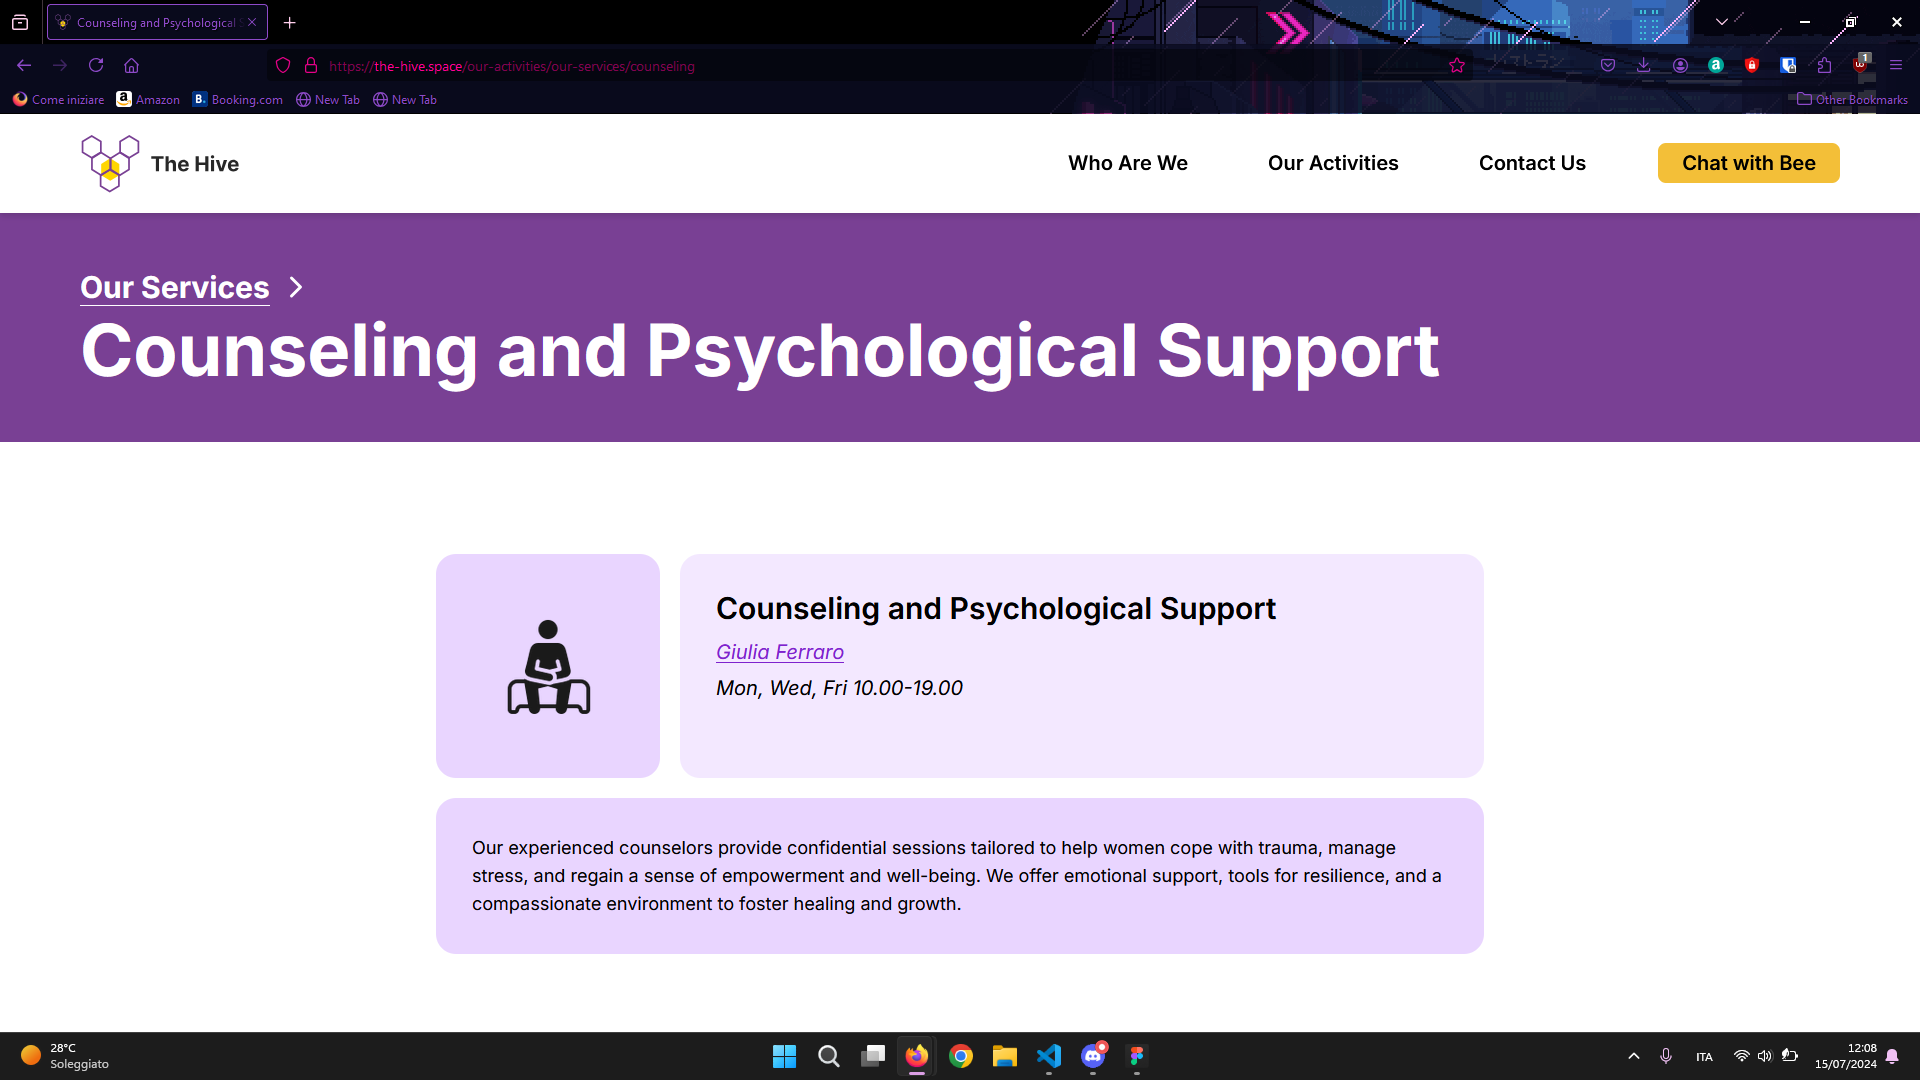
\includegraphics[width=0.5\linewidth]{img/design-document/interaction-scenarios/scenario1/step-5.png}
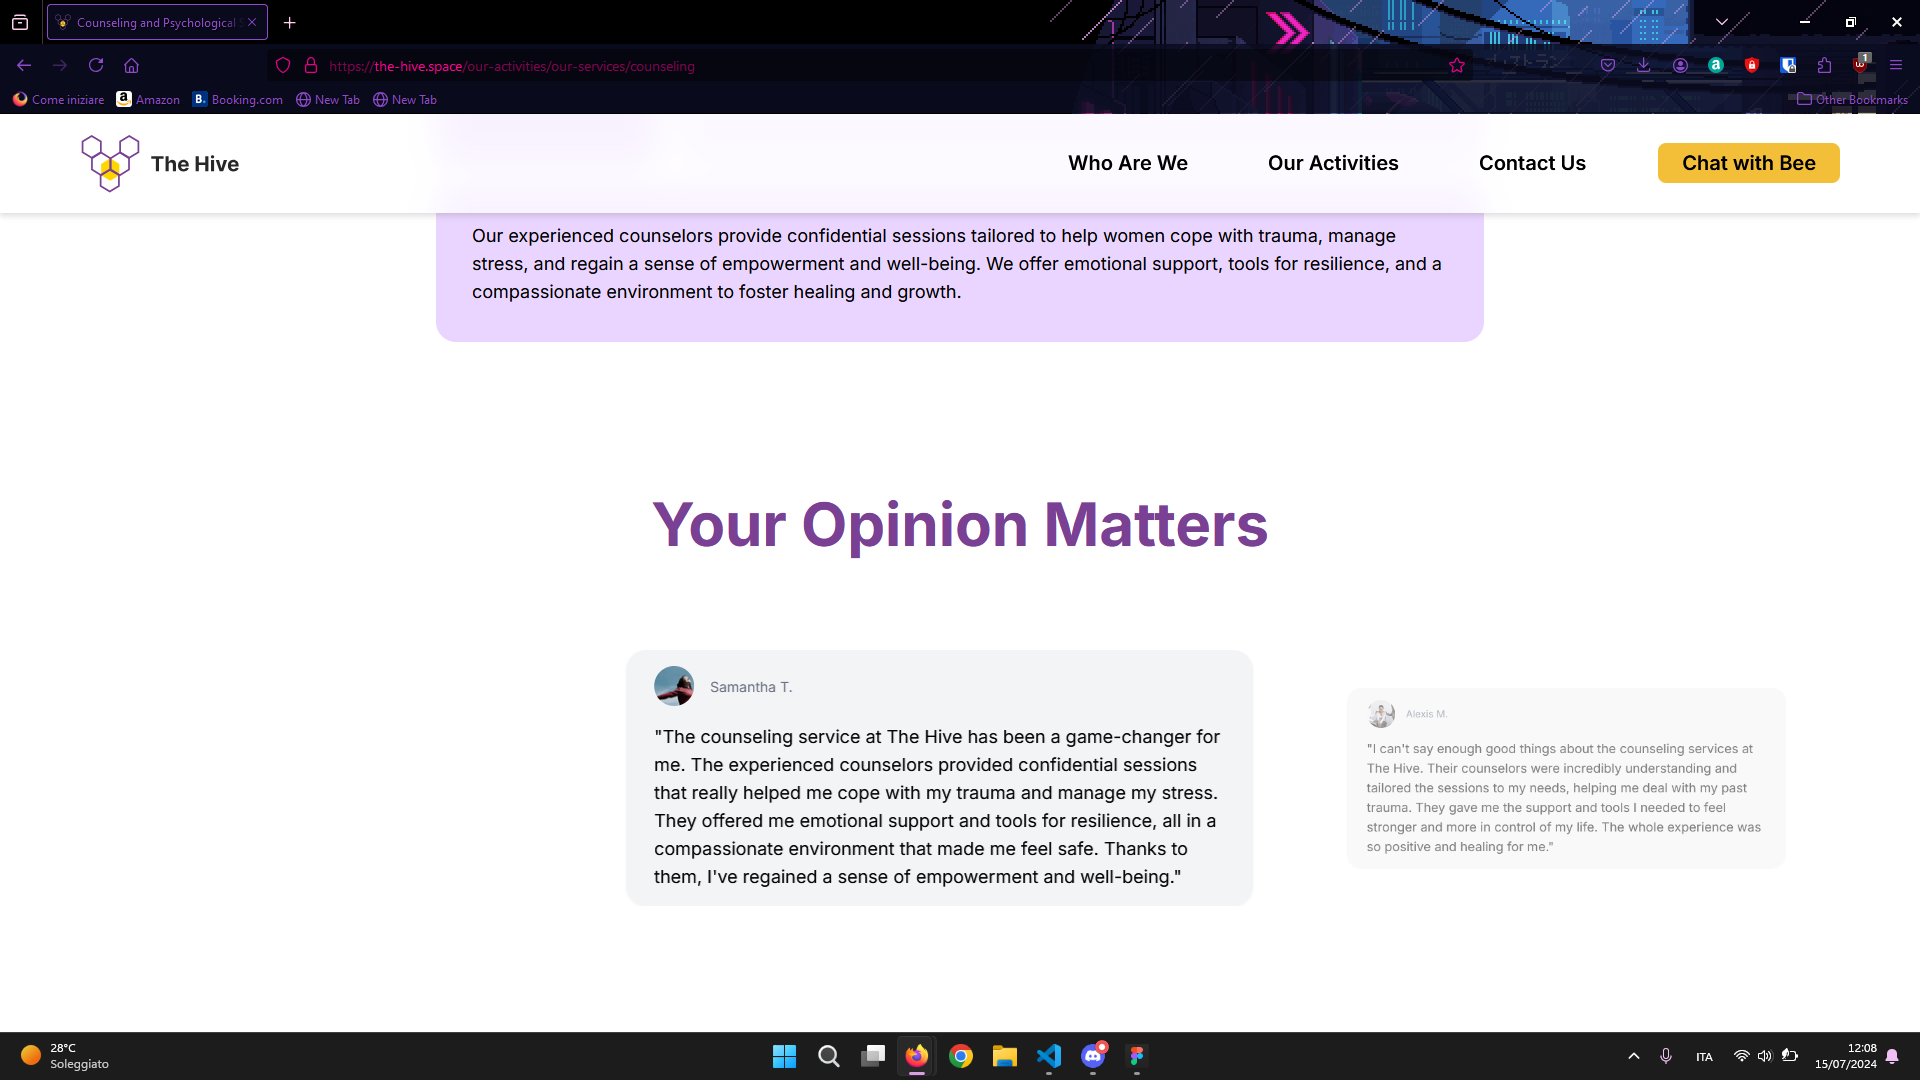
\includegraphics[width=0.5\linewidth]{img/design-document/interaction-scenarios/scenario1/step-6.png}

%Description
\subsection{Scenario 2}
A close friend of Paola S. has been struggling for some time at her workplace because of a colleague’s behavior towards here.
Paola knows that her friend has been consistently belittled and mistreated, and wants to find out how she can help her considering
the situation. She knows about The Hive and remembers that the center has recently added a risk assessing chat bot, so she decides
to try it, in order to better understand the severity of her friend's situation. Once on the homepage of the website she directly
goes for the link to the chatbot on the navigation bar (landmarks).
She chats for a bit with Bee, describing the situation of her friend and answering the questions Bee asks her.
Bee gives her a few suggestions and possible contacts that could help her friend.

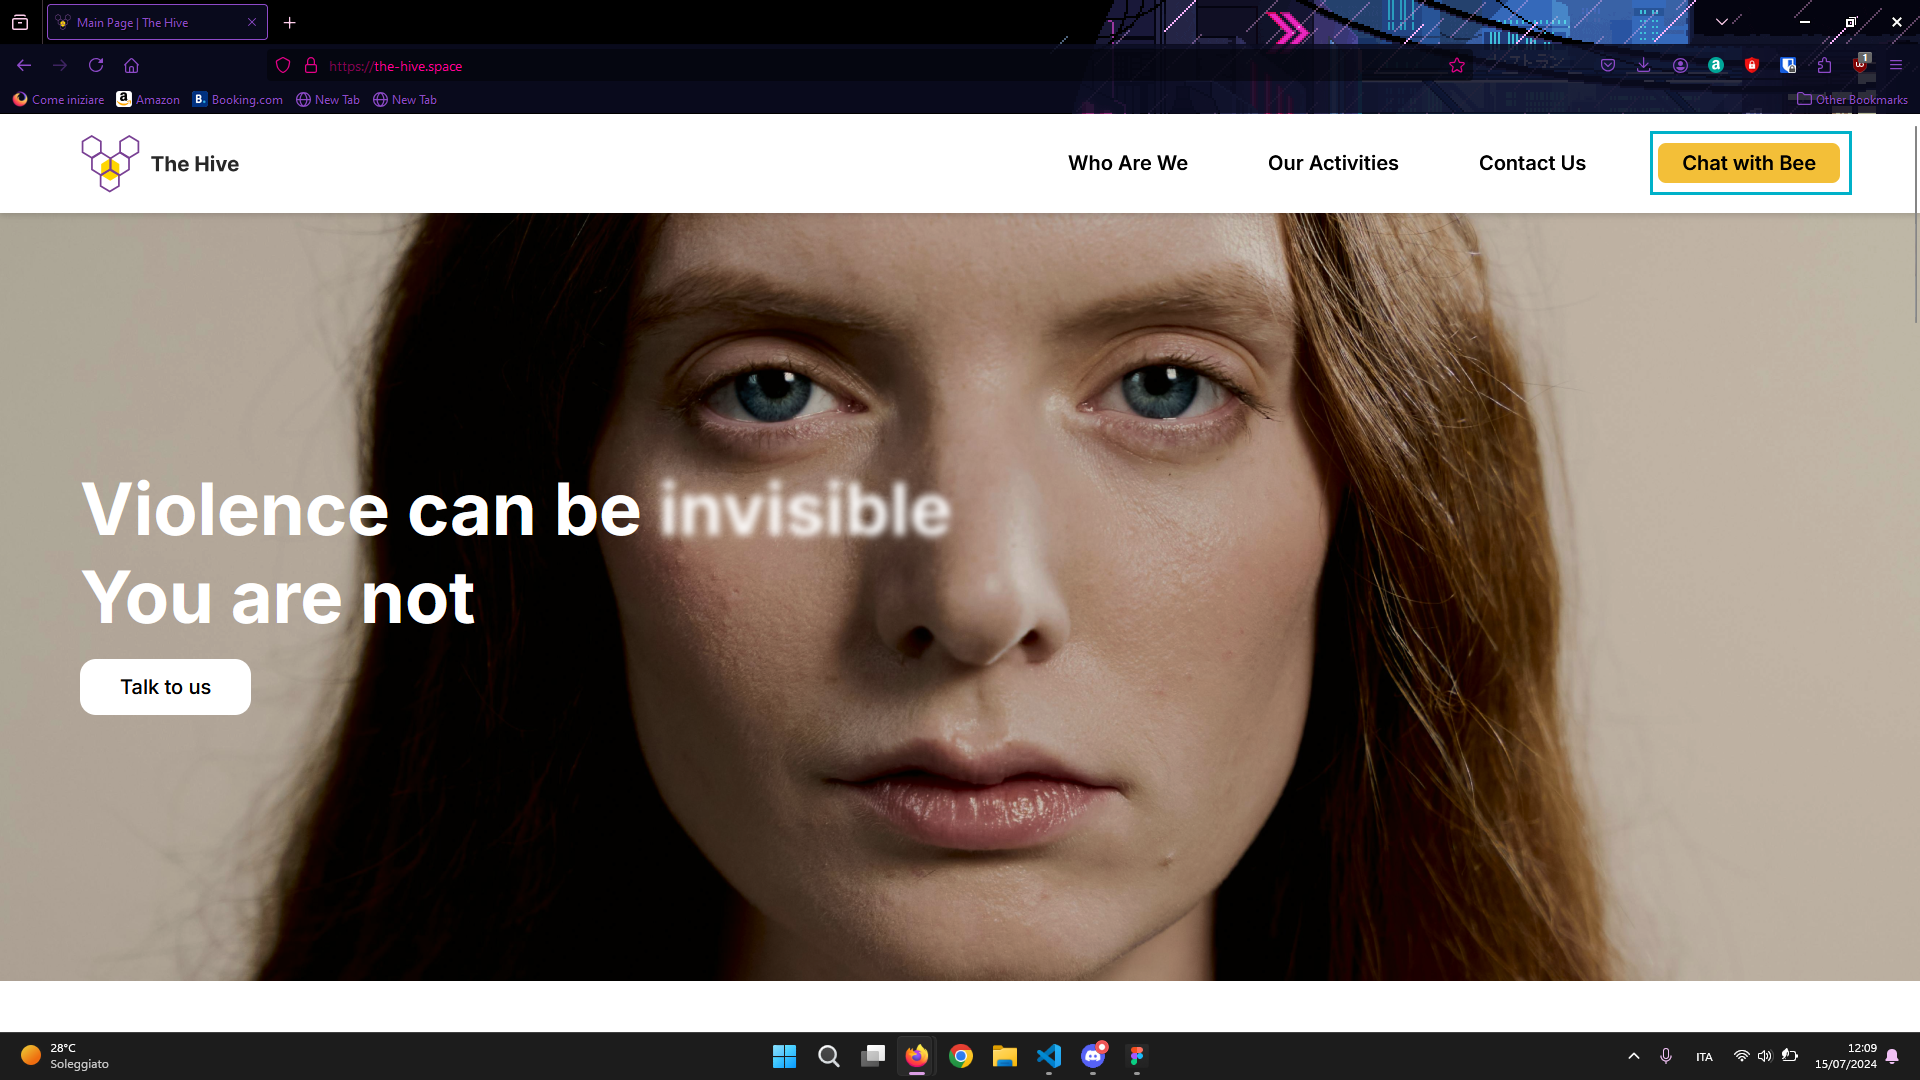
\includegraphics[width=0.5\linewidth]{img/design-document/interaction-scenarios/scenario2/step-1.png}
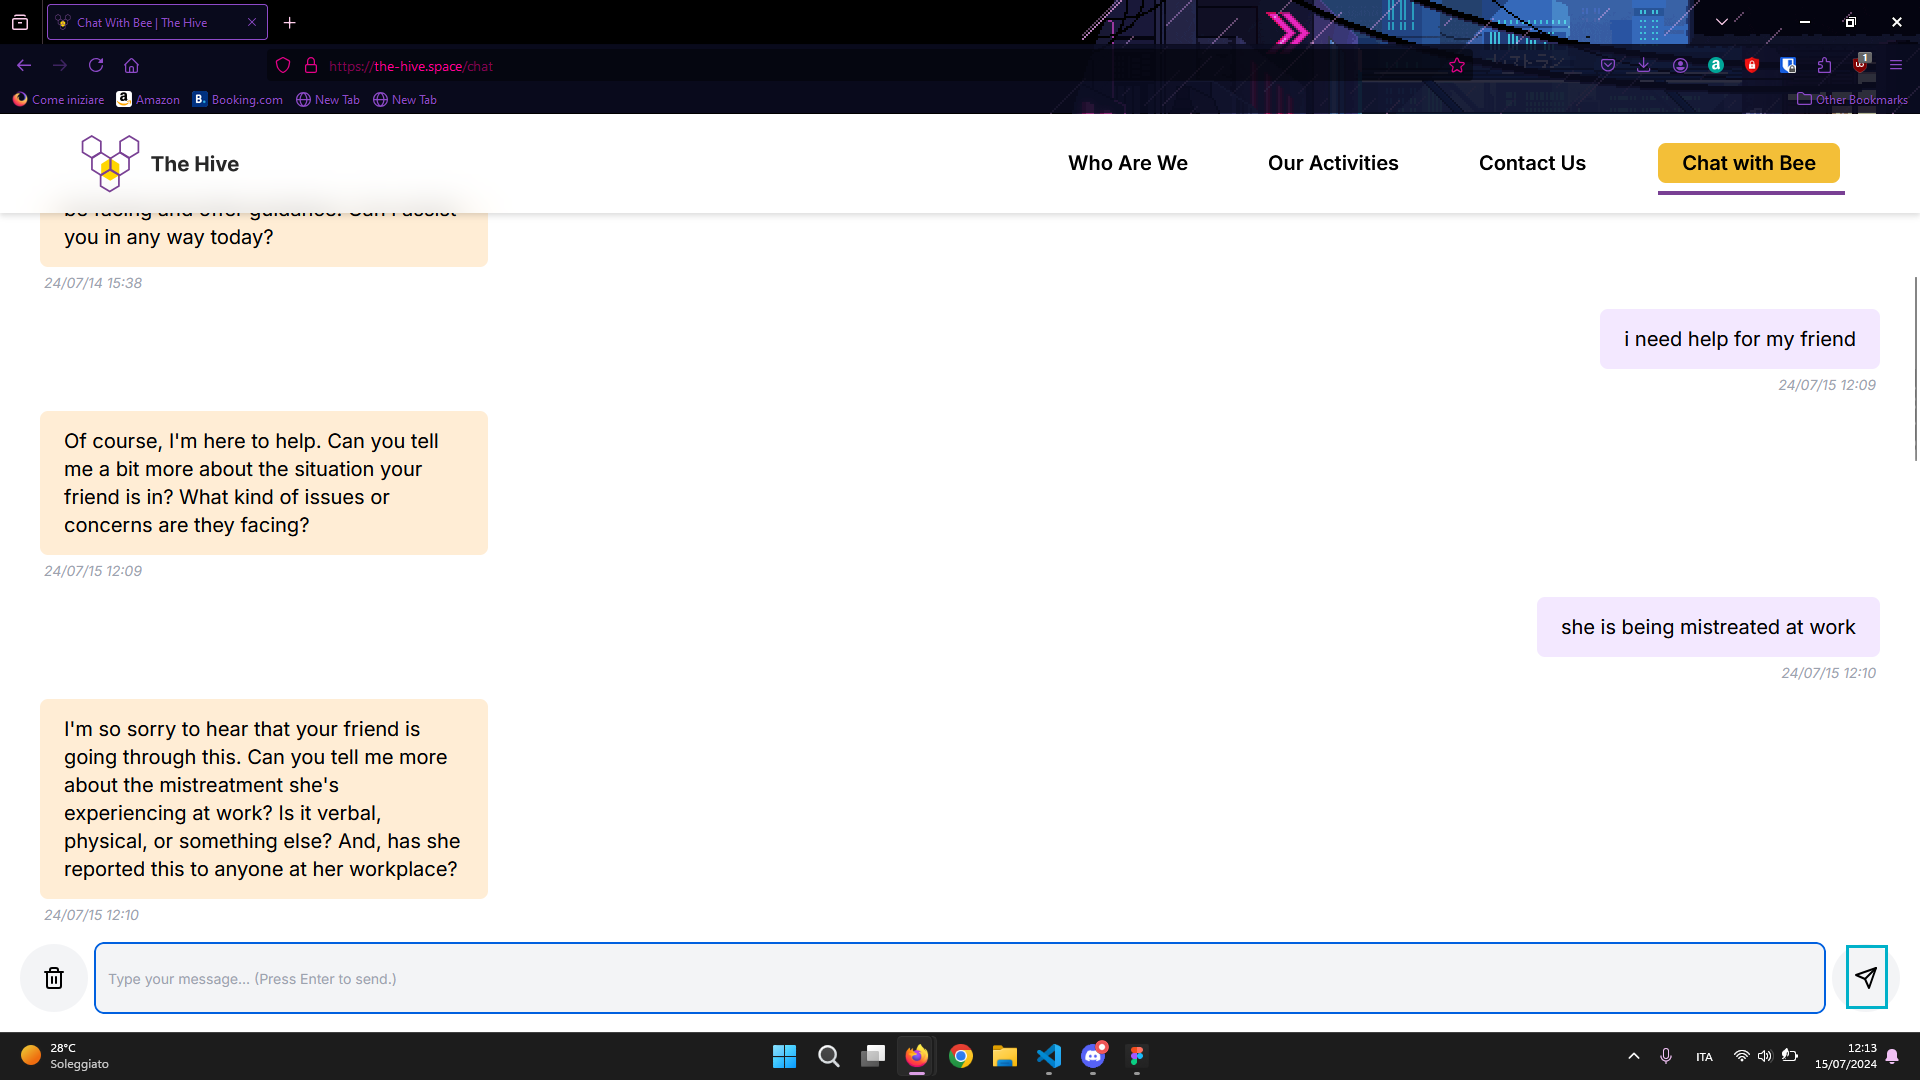
\includegraphics[width=0.5\linewidth]{img/design-document/interaction-scenarios/scenario2/step-2.png}

%Screenshots
\subsection{Scenario 3}
Giovanni L. is the principal of a middle school based in Milan. Recently one of the teachers in his school has mentioned that she
wanted to organize a seminar to sensitize the students about the topic of gender inequality for the occasion of the International
Women’s day. For this purpose she gave him the name of a contact she knows from the center The Hive.  Giovanni goes into the center’s
website and through the navigation bar (landmarks) he easily finds the “Who we are” page. Here he browses to find “Filippo Pantaleone”
(group link), the contact of his colleague, and looks through his Profile page. Utilizing the sidebar links (structural links) he finds
the activities Filippo is responsible for and follows the link to the project “ARYA, To Counter Gender Stereotypes”, which is perfect for
what he’s looking for. He decides then to contact the center through the apposite section on the website.

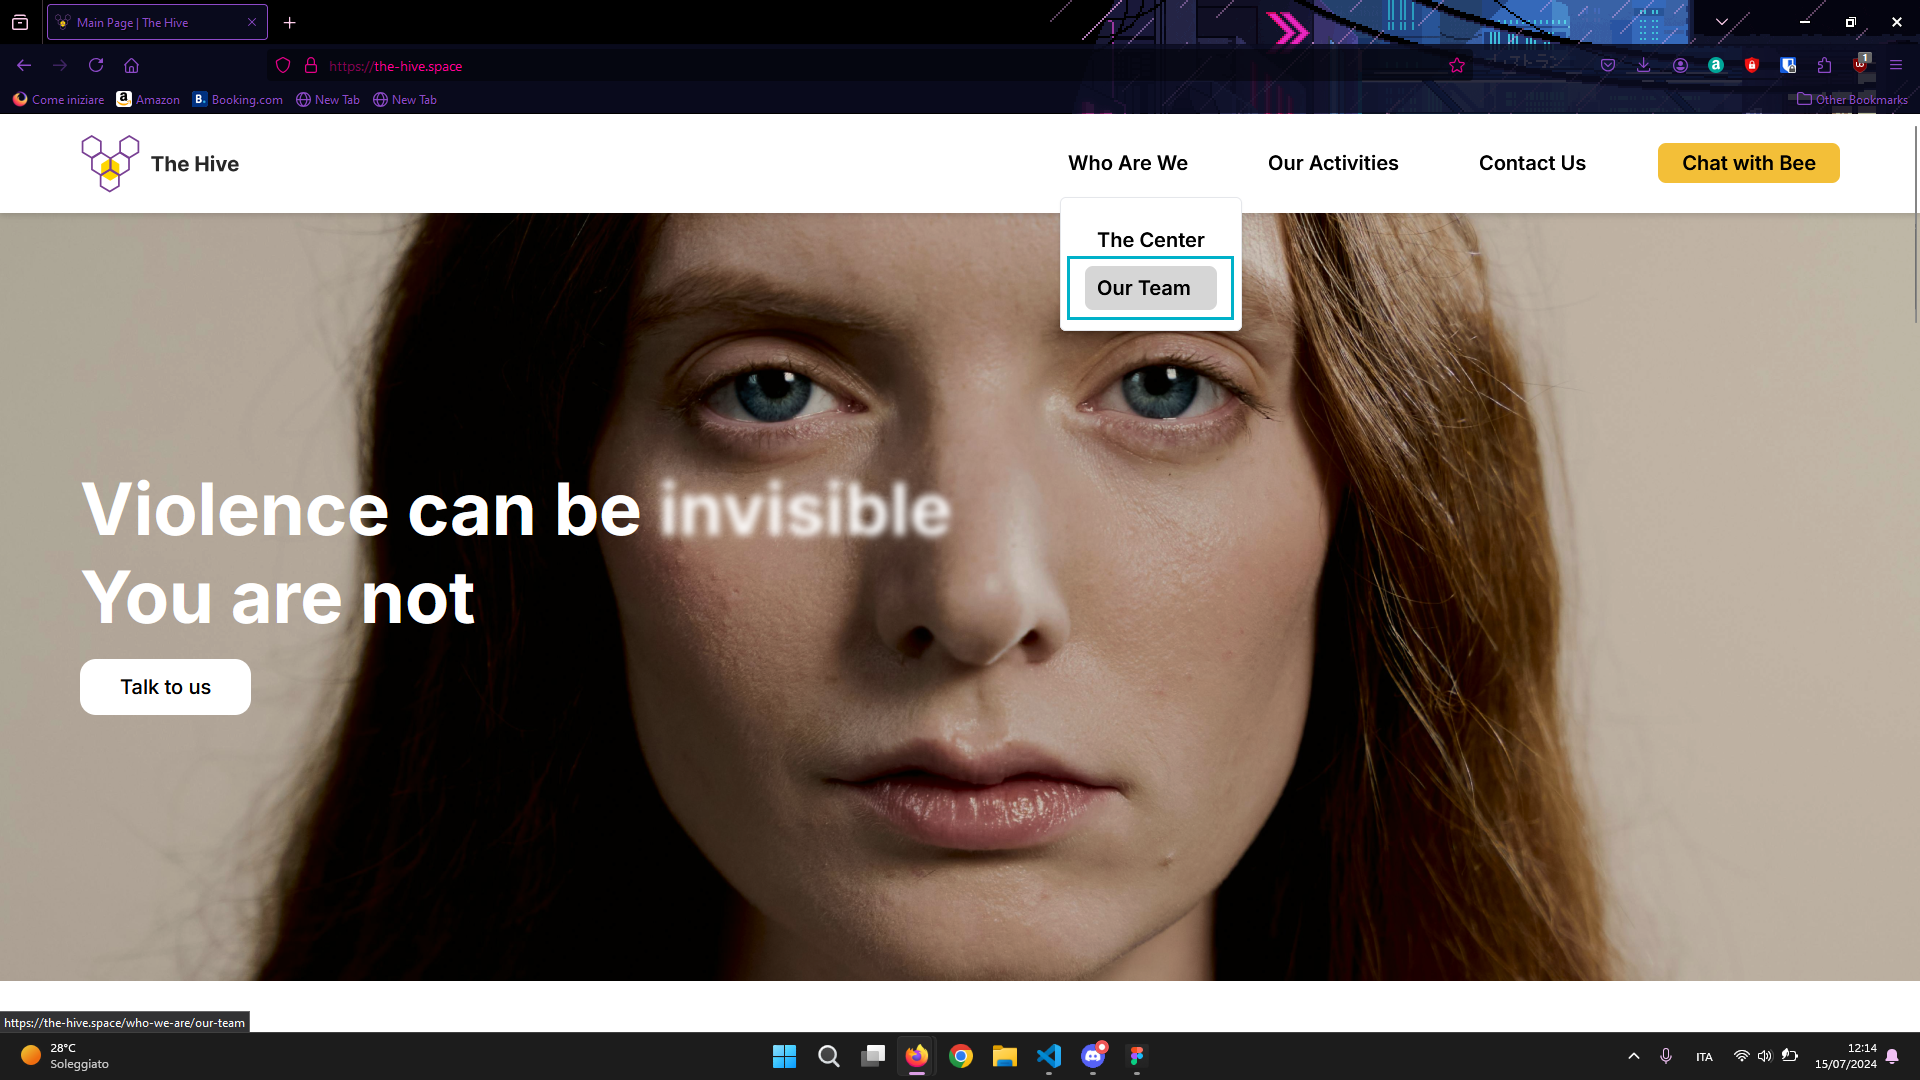
\includegraphics[width=0.5\linewidth]{img/design-document/interaction-scenarios/scenario3/step-1.png}
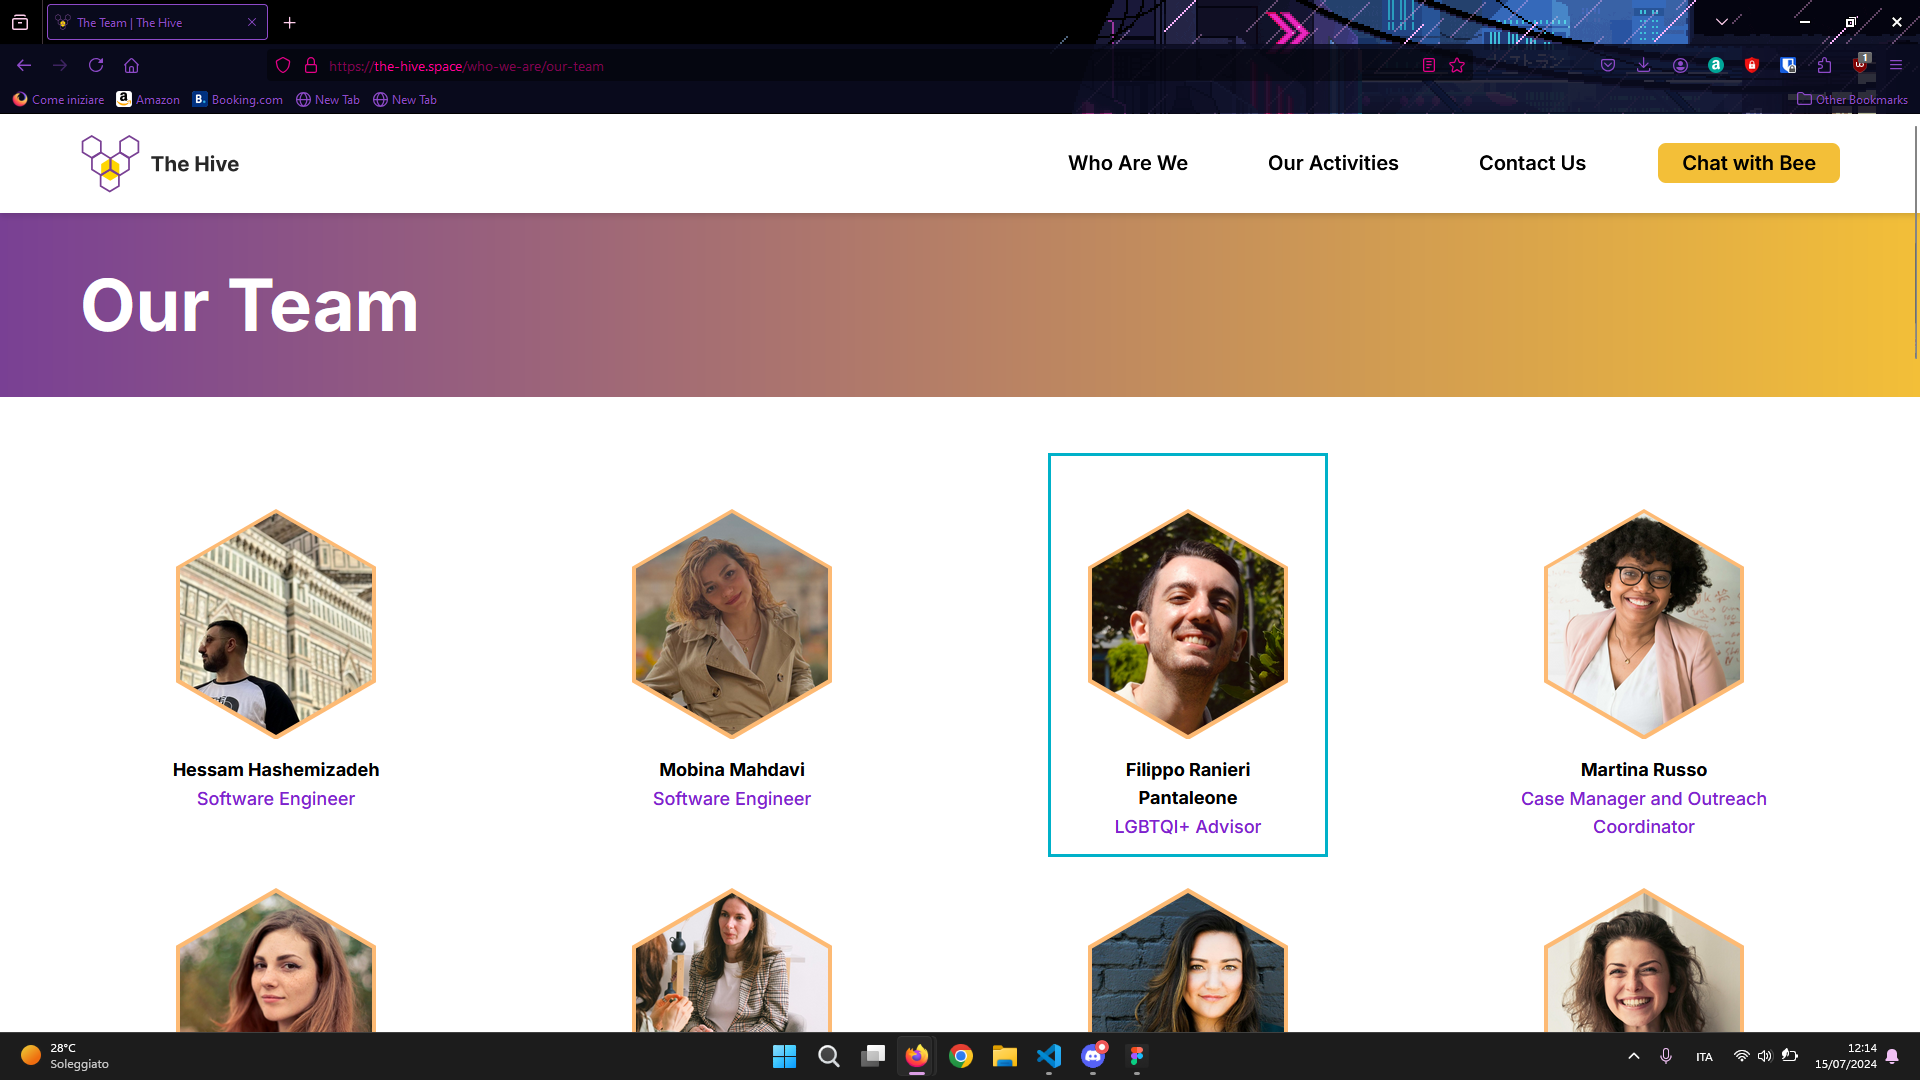
\includegraphics[width=0.5\linewidth]{img/design-document/interaction-scenarios/scenario3/step-2.png}
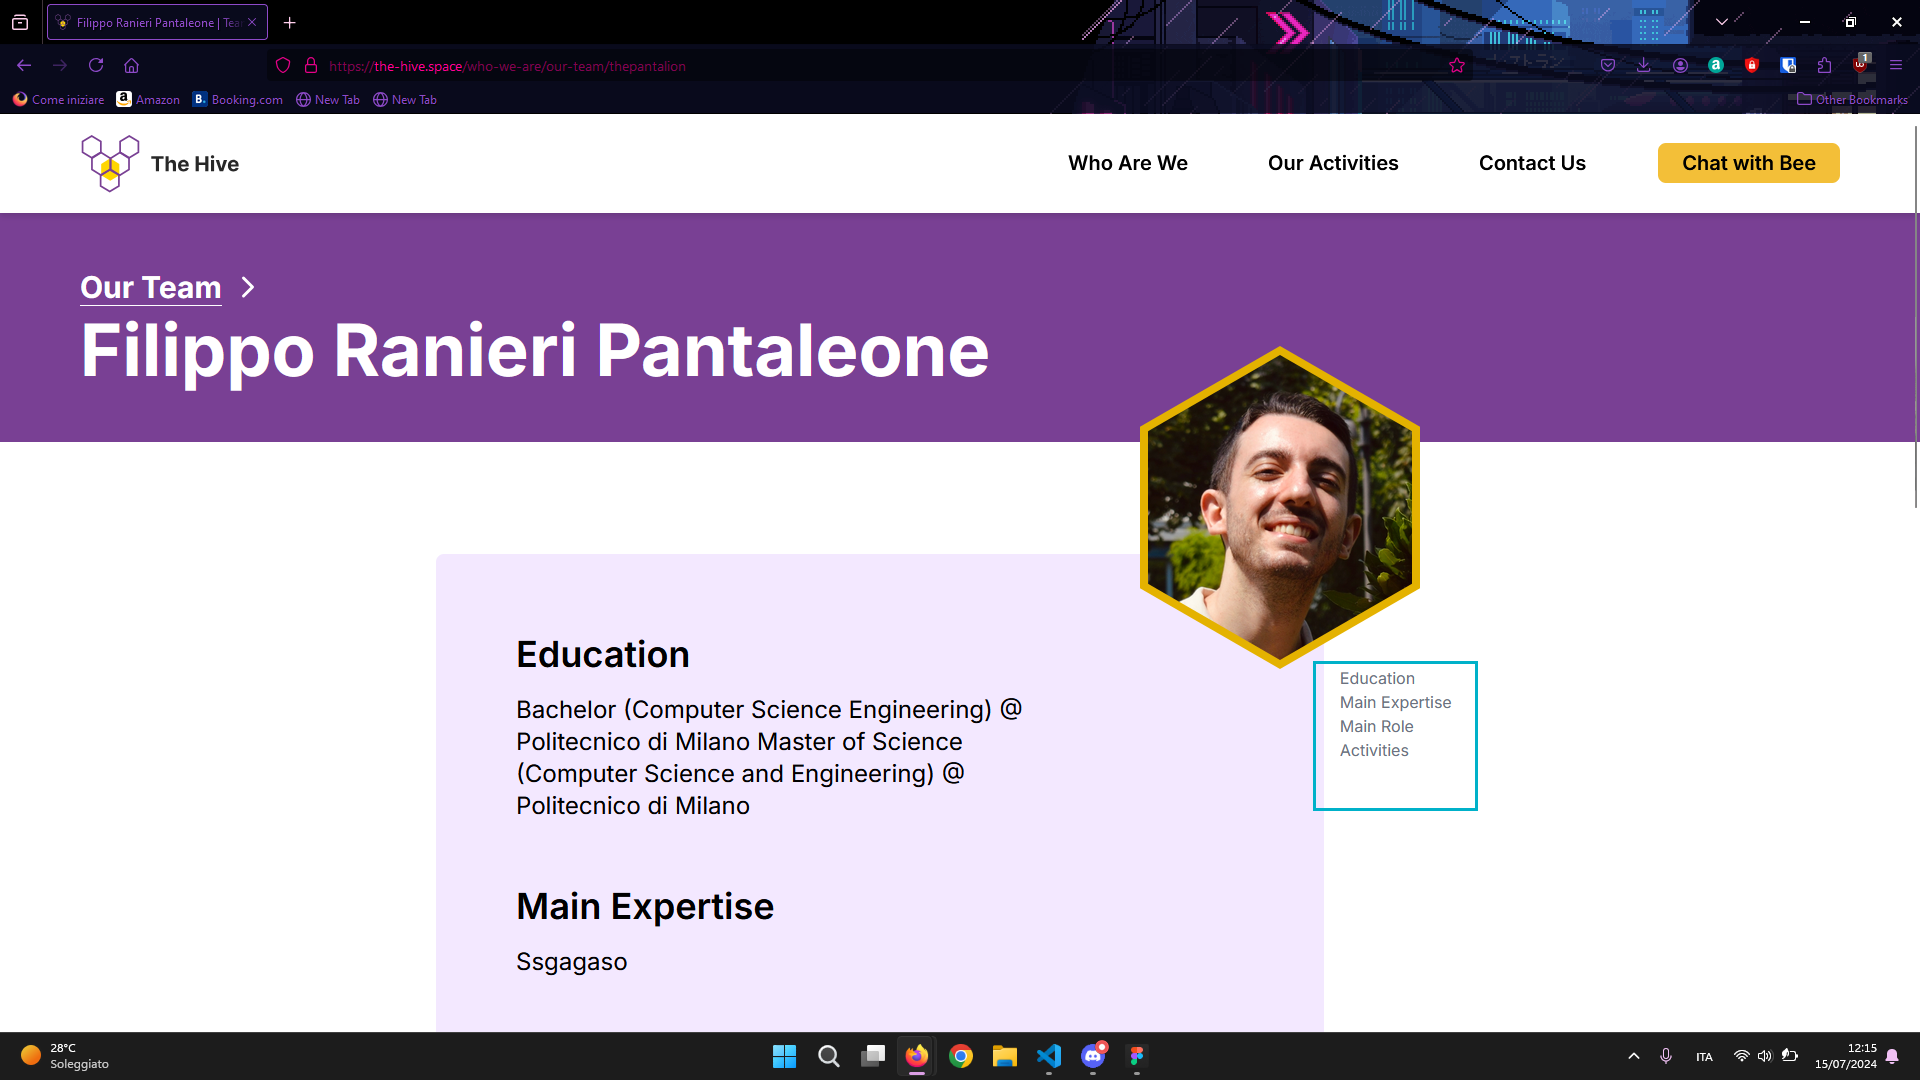
\includegraphics[width=0.5\linewidth]{img/design-document/interaction-scenarios/scenario3/step-3.png}
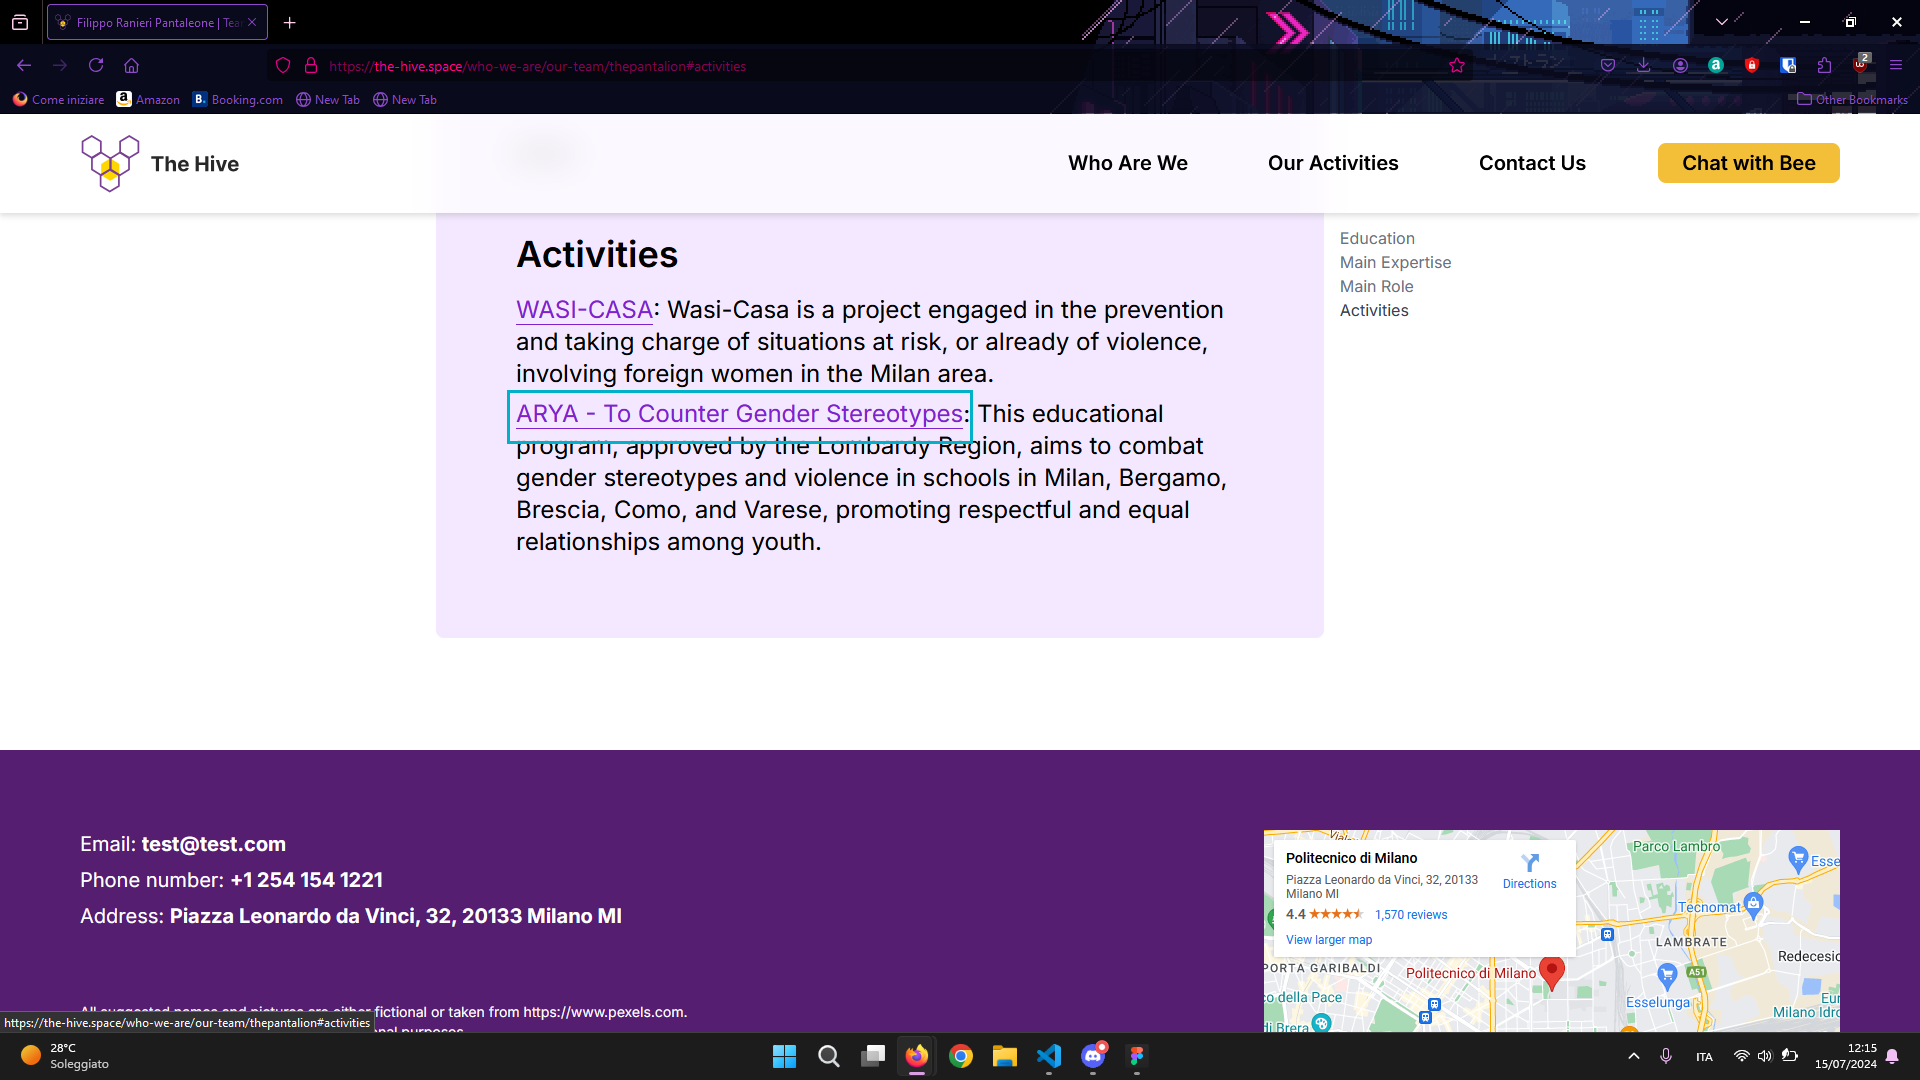
\includegraphics[width=0.5\linewidth]{img/design-document/interaction-scenarios/scenario3/step-4.png}
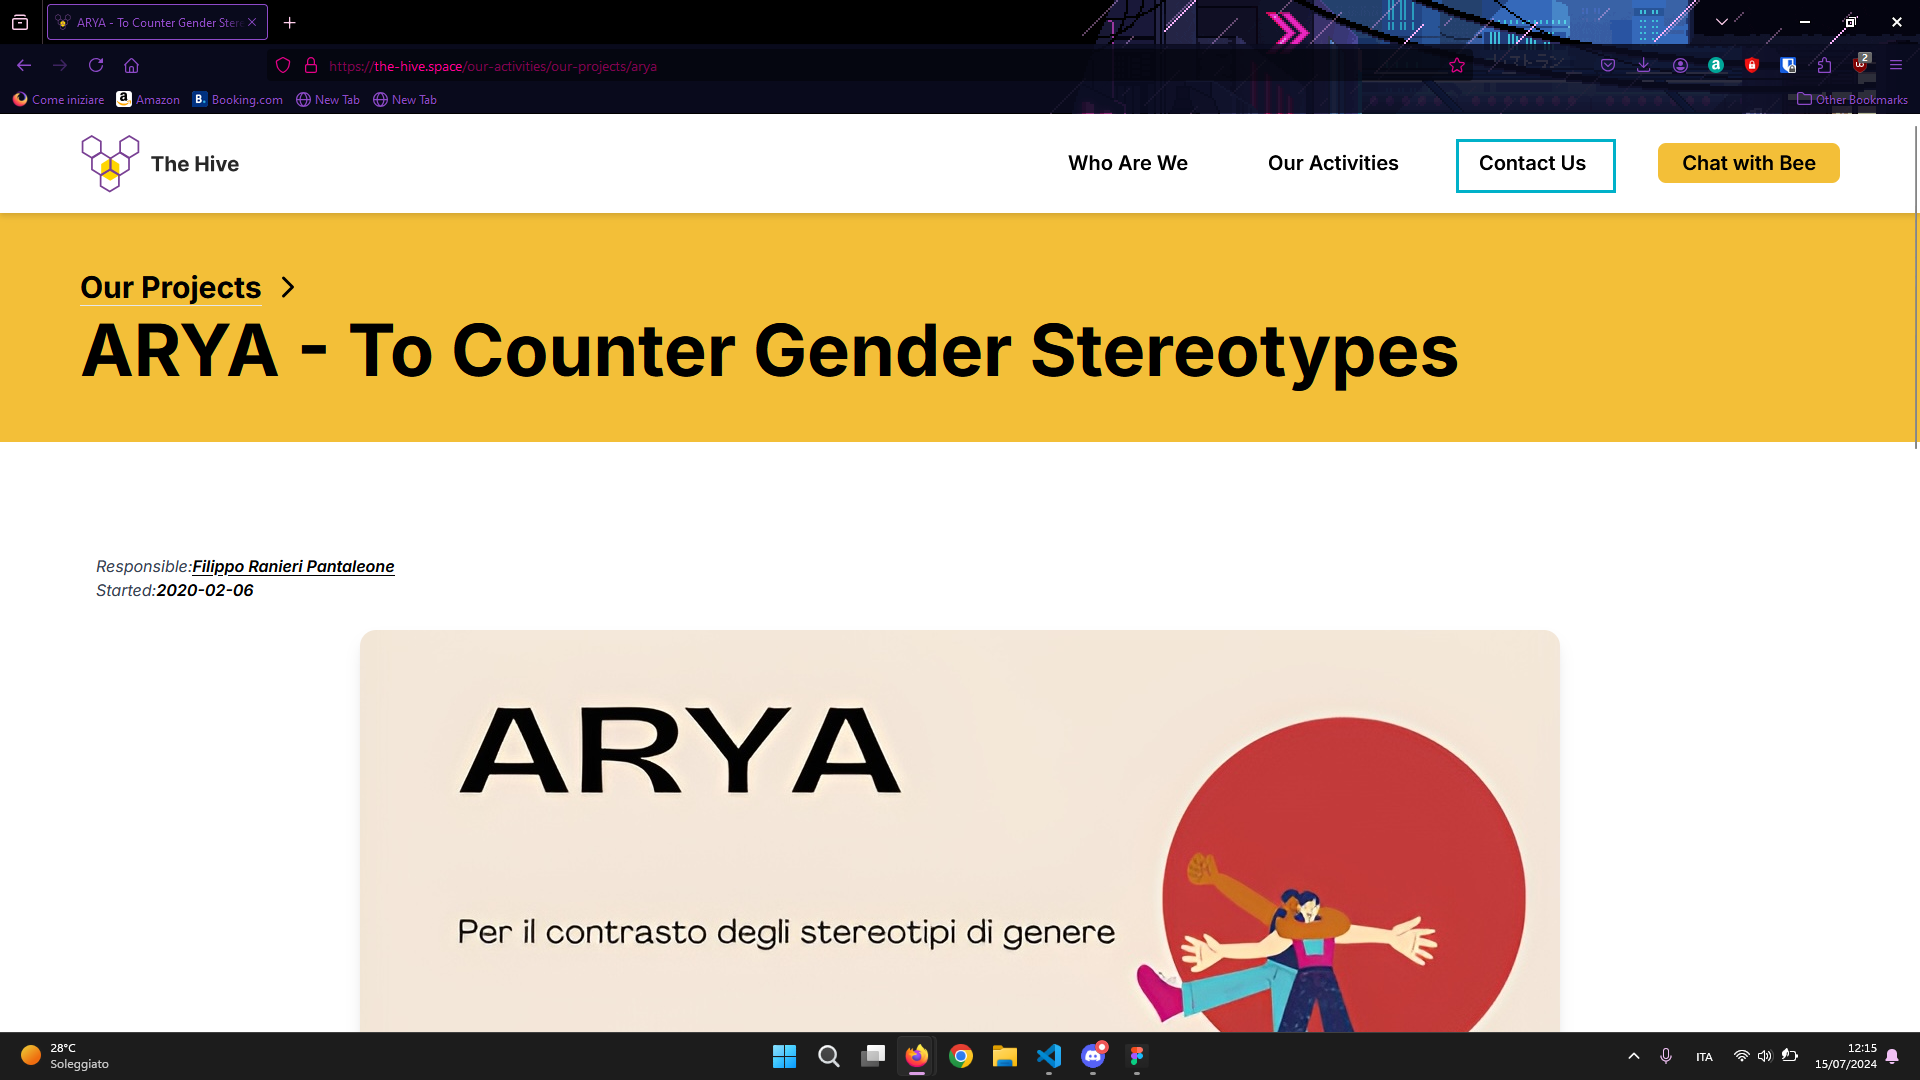
\includegraphics[width=0.5\linewidth]{img/design-document/interaction-scenarios/scenario3/step-5.png}
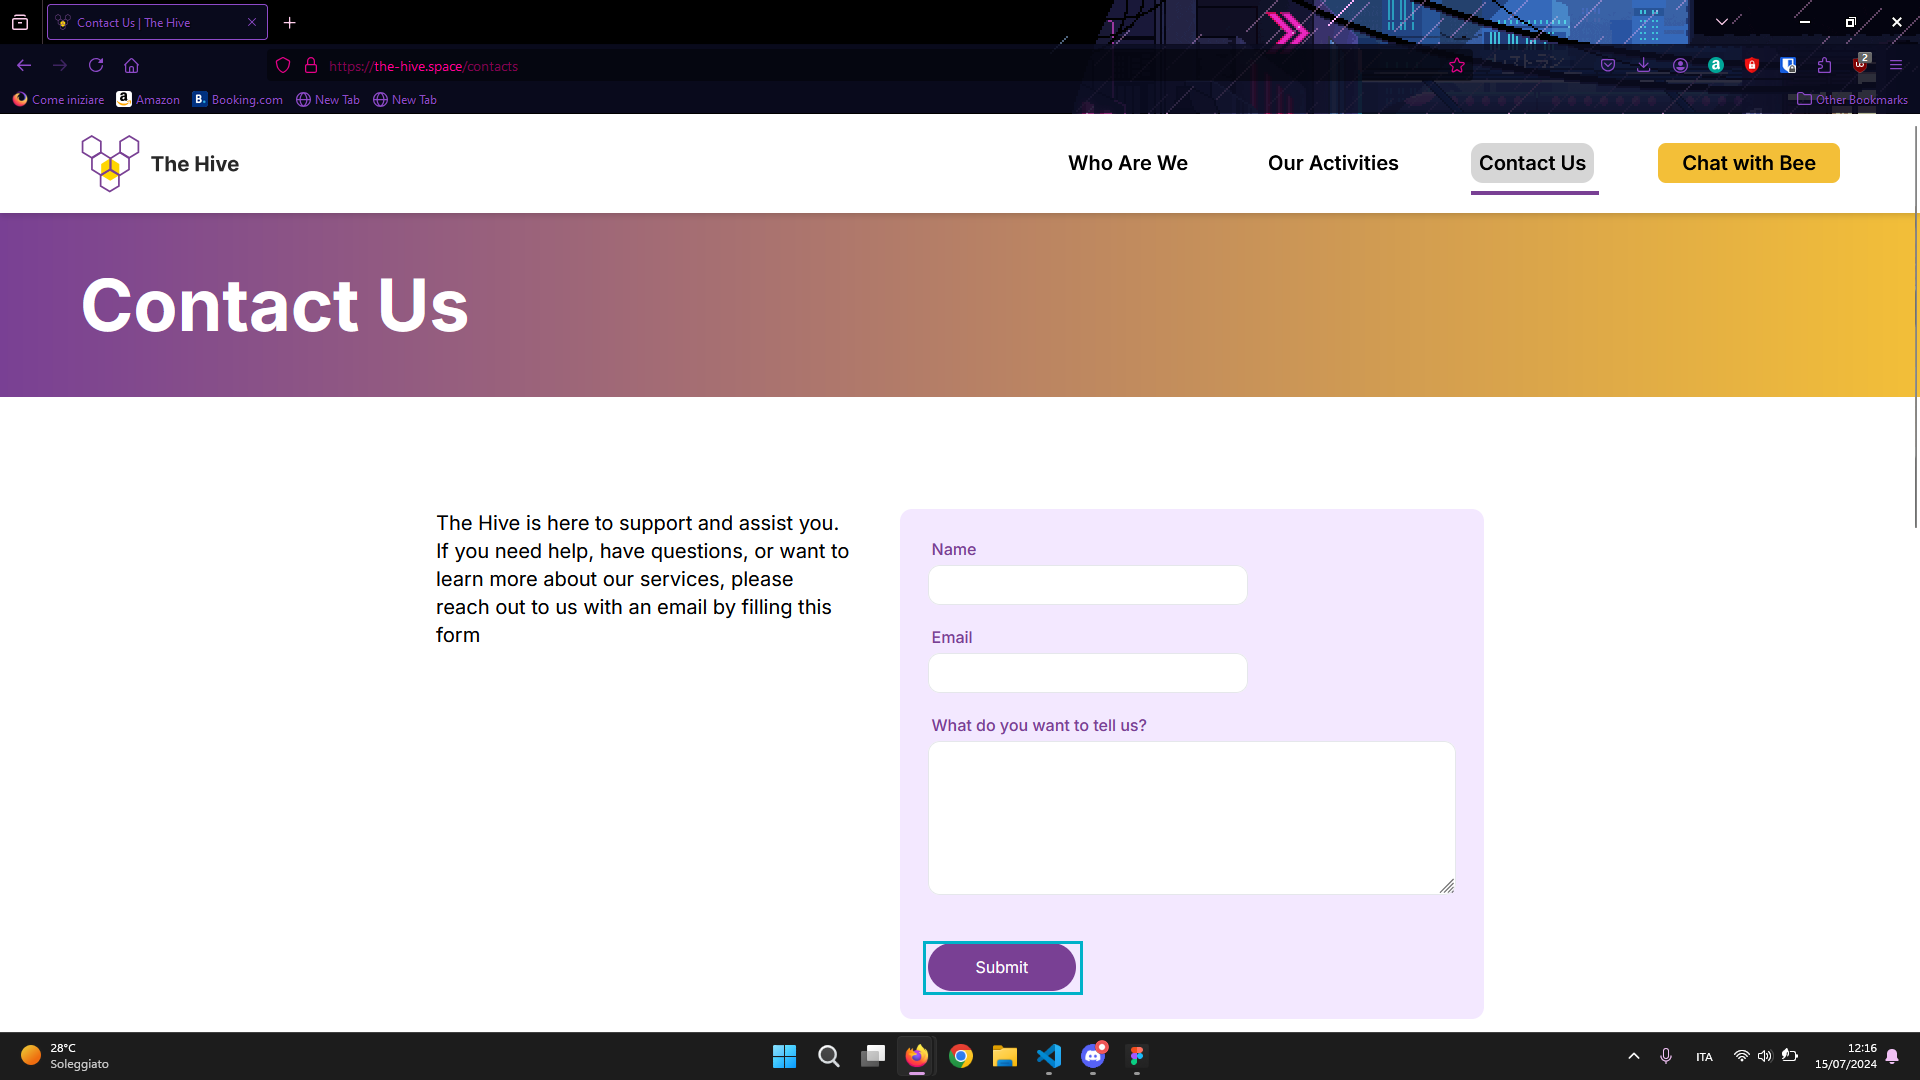
\includegraphics[width=0.5\linewidth]{img/design-document/interaction-scenarios/scenario3/step-6.png}


\pagebreak
\section{DB Design}
\subsection{ER Schema}

% TODO Verify that all design steps are included here
